%%%%%%%%%%%%%%%%%% GENERATED DISSERTATION SOURCE %%%%%%%%%%%%%%%%%%
% Generated from the optimized Markdown copy in final draft.
% Original template files were copied before modification.

\begin{filecontents*}{\jobname.xmpdata}
  \Title{A Two-Layer Decision-Making System for Vehicle Lane Changing Based on Reinforcement Learning}
  \Author{14226506}
  \Language{en-GB}
  \Copyrighted{True}
\end{filecontents*}

\documentclass[11pt,msc]{uom_eee_dissertation_casson}

\usepackage{graphicx}
  \graphicspath{ {./images/} }
\usepackage{amsmath}
  \allowdisplaybreaks[1]
\usepackage{amssymb}
\usepackage{url}
\usepackage{float}
\usepackage{booktabs}
\usepackage{longtable}
\usepackage{supertabular}
\usepackage{array}
\usepackage{tabularx}
\usepackage{multirow}
\usepackage{subcaption}
\usepackage{siunitx}
\usepackage[base]{babel}

\newcommand{\degree}{\ensuremath{^\circ}}
\newcommand{\sus}[1]{$^{\mbox{\scriptsize #1}}$}
\newcommand{\sub}[1]{$_{\mbox{\scriptsize #1}}$}
\newcommand{\otoprule}{\midrule[\heavyrulewidth]}
\newcolumntype{Z}{>{\centering\arraybackslash}X}
\newcolumntype{L}[1]{>{\RaggedRight\arraybackslash\hspace{0pt}}p{#1}}
\setlength{\emergencystretch}{3em}
\hbadness=10000
\setlength{\LTpre}{0pt}
\setlength{\LTpost}{0pt}

\usepackage[style=ieee,backend=biber,backref=true,hyperref=auto,maxbibnames=3,minbibnames=1]{biblatex}
\DefineBibliographyStrings{english}{backrefpage = {cited on p\adddot}, backrefpages = {cited on pp\adddot}}
\addbibresource{references.bib}

% Compact settings for the final dissertation copy.
\titlespacing*{\section}{0pt}{1.0ex plus 0.2ex minus 0.2ex}{0.45ex}
\titlespacing*{\subsection}{0pt}{0.75ex plus 0.2ex minus 0.2ex}{0.25ex}
\titlespacing*{\subsubsection}{0pt}{0.55ex plus 0.15ex minus 0.15ex}{0.15ex}
\captionsetup{font=small,skip=1pt}
\captionsetup[figure]{font=small,skip=1pt}
\setlength{\textfloatsep}{3pt plus 1pt minus 1pt}
\setlength{\floatsep}{3pt plus 1pt minus 1pt}
\setlength{\intextsep}{3pt plus 1pt minus 1pt}
\setlength{\abovedisplayskip}{2pt plus 1pt minus 1pt}
\setlength{\belowdisplayskip}{2pt plus 1pt minus 1pt}
\setlength{\abovedisplayshortskip}{1pt plus 1pt minus 1pt}
\setlength{\belowdisplayshortskip}{1pt plus 1pt minus 1pt}
\setlength{\tabcolsep}{3pt}
\renewcommand{\arraystretch}{0.82}
\AtBeginEnvironment{equation}{\footnotesize\singlespacing}
\AtBeginEnvironment{longtable}{\footnotesize\singlespacing}

\begin{document}
\makeatletter
\title{\xmp@Title}
\studentid{\xmp@Author}
\makeatother

\course{Robotics}
\faculty{Science and Engineering}
\school{School of Engineering}
\submitdate{2026}
\wordcount{4,217}
\maketitle

\uomtoc

\begin{abstract}
Lane changing is a fundamental problem in autonomous driving. This dissertation proposes a two-layer decision-making and control framework for autonomous vehicles merging into a target lane. The framework separates strategic decision dynamics from physical execution. The high-level decision-making layer contains two opinion variables: a longitudinal opinion that selects a local gap from nearby target-lane vehicles, and a lateral opinion that determines whether the ego vehicle should commit to the selected gap. The longitudinal module observes the three target-lane vehicles closest to the ego vehicle, forms two candidate gaps, evaluates their relative confidence, and accumulates a temporally smoothed preference through nonlinear opinion dynamics. The lateral module evaluates the selected gap using its size and rate of change, uses a Soft Actor-Critic (SAC) policy to generate the attention intensity, and maps the resulting opinion to continuous target points. The low-level controller then combines safety avoidance, target tracking, and a proportional-integral-derivative (PID)-like physical input law to generate acceleration and steering-rate commands.

Simulation experiments are implemented in Python in two environments. The single-gap environment contains one front vehicle, one rear vehicle, and one merging ego vehicle with a randomized initial longitudinal position; the rear vehicle creates a yielding opportunity after 20 s. The multi-gap environment contains five target-lane vehicles and four dynamically changing gaps over a 40 s horizon. In the single-gap tests, the SAC attention policy achieves an average episodic reward of 233.4 compared with 115.8 for the radial-basis-function (RBF) baseline, completes the task in 6.9 s rather than 29.45 s, and maintains zero collisions. In multi-gap deployment, the single-gap policy maintains a success rate of approximately 97\%, and the opinion-based high-level selector improves mean reward by 55.3\% over the simple max-score selector.
\end{abstract}
\clearpage

\begin{uomoriginality}
  \uomoriginalitydeclaration
\end{uomoriginality}
\uomcopyrightstatement

\uomstartmainbody

\section{Introduction}

\subsection{Background and Motivation}

\subsubsection{Decision-making strategies for merge and lane-change interaction}

Lane-changing decisions are representative problems in autonomous driving. A lane change changes the available gaps, right-of-way expectations, and future responses of surrounding vehicles. Recent research has therefore treated lane changing as an interactive decision problem rather than a purely geometric path-planning task. Game-theoretic models are widely used because they explicitly describe the strategic relationship between the ego vehicle and surrounding vehicles. Lane-changing intention, collision probability, and dynamic risk can be incorporated into a payoff function to evaluate whether a manoeuvre is beneficial or dangerous \cite{R1,R2}. Physics-inspired methods, such as molecular interaction potential models, further express attraction and repulsion between vehicles as continuous interaction forces \cite{R3}. Other studies consider incomplete information and social driving preferences, because surrounding human-driven vehicles may behave cooperatively, aggressively, or uncertainly in merging conflicts \cite{R4}.

Learning-based interactive prediction provides a second route. Graph neural networks and attention mechanisms represent vehicles as nodes and inter-vehicle influence as edges or attention weights. This representation is suitable for lane changing, where the number and importance of surrounding vehicles vary over time. Existing studies use topological graphs with driving behaviour and traffic context to predict lane-changing intentions \cite{R5}, while plan-aware graph attention models predict how surrounding vehicles respond to candidate ego intentions before generating a trajectory \cite{R6}. These studies show that interaction modelling should estimate not only where other vehicles will move, but also how they may respond to the ego decision. Cooperative control methods provide a third route. In connected autonomous driving, surrounding vehicles can create gaps, coordinate lane-changing order, or maintain fleet stability \cite{R7,R8}. Together, these studies motivate a hierarchical framework that combines strategic interaction modelling, adaptive decision dynamics, and safe execution.

\subsubsection{Reinforcement learning for adaptive decision dynamics}

Lane-changing decisions are sequential, uncertain, and feedback driven. A vehicle must decide when to wait, when to merge, and how strongly to commit. Fixed-parameter controllers may work in static cases, but they often lack flexibility when traffic states change or when the system must move between cautious waiting and active merging. Deep reinforcement learning (DRL) provides a mechanism for learning decision strategies through repeated interaction. Existing studies have integrated safety rules, future-risk assessment, reward shaping, and robust observation modelling into DRL lane-changing strategies \cite{R9,R10,R11}. These studies suggest that reinforcement learning (RL) should not be used as an unconstrained black box; instead, it should be constrained by interpretable states, safety-aware rewards, and model-based structure.

Multi-agent reinforcement learning (MARL) further allows connected or autonomous vehicles to learn from neighbouring vehicles while considering system-level outcomes such as traffic efficiency, comfort, and safety \cite{R12}. Right-of-way coordination and Mix Q-learning show that lane changing can balance individual and group benefits \cite{R13,R14}. For this dissertation, these studies support a specific use of RL: the learned policy does not directly output lane-changing motion, but adjusts the attention parameter inside a nonlinear opinion-dynamics model. The decision remains interpretable, while the timing and strength of commitment can adapt to the environment.

\subsubsection{Evaluation dimensions: from efficiency to safety, comfort, and adaptability}

The evaluation of lane-changing decisions has shifted from single efficiency metrics to multidimensional assessment. Average speed, travel time, traffic volume, and lane-changing success rate remain important, but they are insufficient for safety-critical autonomous driving. A rapid lane change may still be unsafe, uncomfortable, or disruptive to traffic flow. Recent studies therefore evaluate collision risk, minimum distance, braking feasibility, safety violation rate, acceleration, traffic-flow stability, and robustness under perception uncertainty \cite{R7,R8,R10,R15}. This project follows these evaluation dimensions by measuring task progress, completion time, collision behaviour, minimum distance, reward, and switching stability.

\subsection{Aims and Objectives}

The aim of this project is to develop, integrate, and evaluate a two-layer decision-making and control framework for interactive autonomous lane merging. The framework uses nonlinear opinion dynamics to represent strategic commitment, RL to adapt the lateral attention intensity, and a safety-aware low-level controller to convert opinion states into physical vehicle inputs.

This project has five objectives. First, it formulates a continuous opinion-dynamics model for longitudinal gap selection and lateral merging commitment. Second, it trains a SAC agent to adjust the lateral attention parameter of the opinion model. Third, it designs a low-level execution controller that combines safety avoidance with front-axle target tracking. Fourth, it implements the complete controller in a Python simulation framework. Fifth, it compares the proposed method with RBF and max-score baselines to evaluate efficiency, safety, and generalization.

\subsection{Scenario and Modeling}

The studied scenario is a lane-merging task in which one ego vehicle travels in the original lane and attempts to merge into a target lane containing continuous traffic. The target-lane vehicles are assumed to be observable through their longitudinal positions and velocities. The ego vehicle does not control these vehicles; instead, it observes their motion, selects a feasible local gap, and generates its own control input. In the single-gap environment, the target lane contains one front vehicle and one rear vehicle. In the multi-gap environment, it contains five vehicles, which form four candidate physical gaps. The ego initial longitudinal position is randomized to test whether the controller can tolerate different entry alignments.

The vehicle model is represented by a front-axle kinematic bicycle abstraction. The ego state contains its planar position, heading, and forward speed, while the physical input consists of longitudinal acceleration and steering-rate commands. The front-axle point is used for decision and tracking because it gives a direct geometric reference for entering a target-lane gap. The high-level decision layer determines the desired gap and merge commitment, and the low-level controller converts the corresponding target point into actual acceleration and angular-rate changes under collision-avoidance constraints.

\begin{figure}[!htbp]
\centering
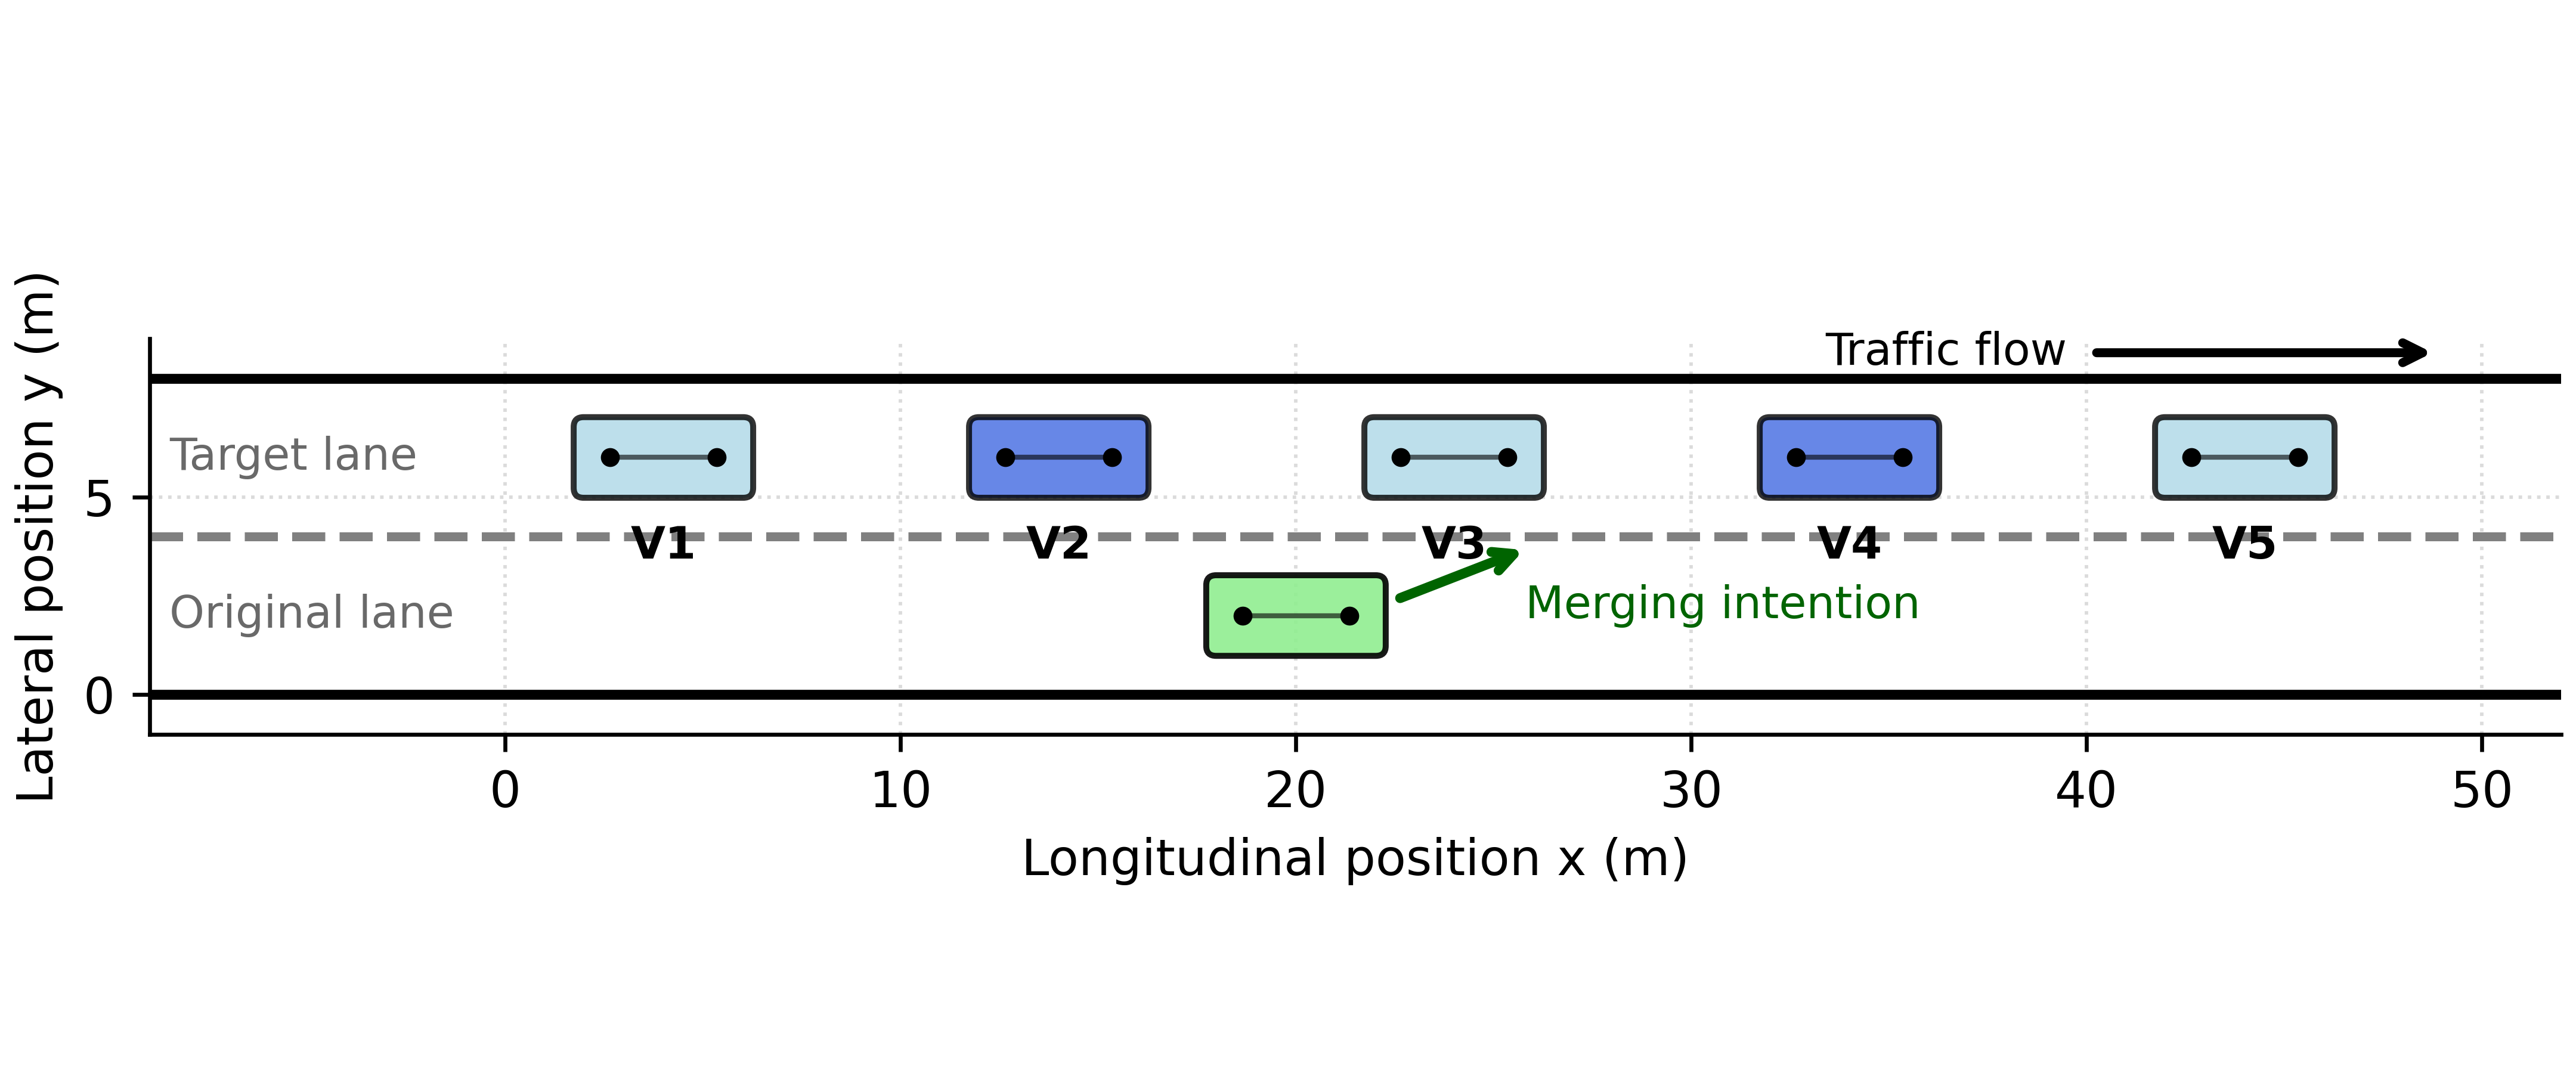
\includegraphics[width=0.60\linewidth]{chapter_1_3_lane_change_scene.png}
\caption{Lane-Merging Scenario Illustration}
\label{fig:lane-merging-scenario-illustration}
\end{figure}

\section{Methods}

The proposed system contains two layers. The high-level decision-making layer includes both longitudinal and lateral opinion dynamics. The longitudinal opinion \(y(t)\) chooses whether the ego vehicle should bias its attention toward a forward or rear candidate gap, and the lateral opinion \(z(t)\) determines how strongly the ego vehicle should move from the original lane toward the selected gap. The low-level control layer does not make a new strategic decision; it converts the target implied by the high-level opinions into safety-aware physical inputs.

\begin{figure}[!htbp]
\centering
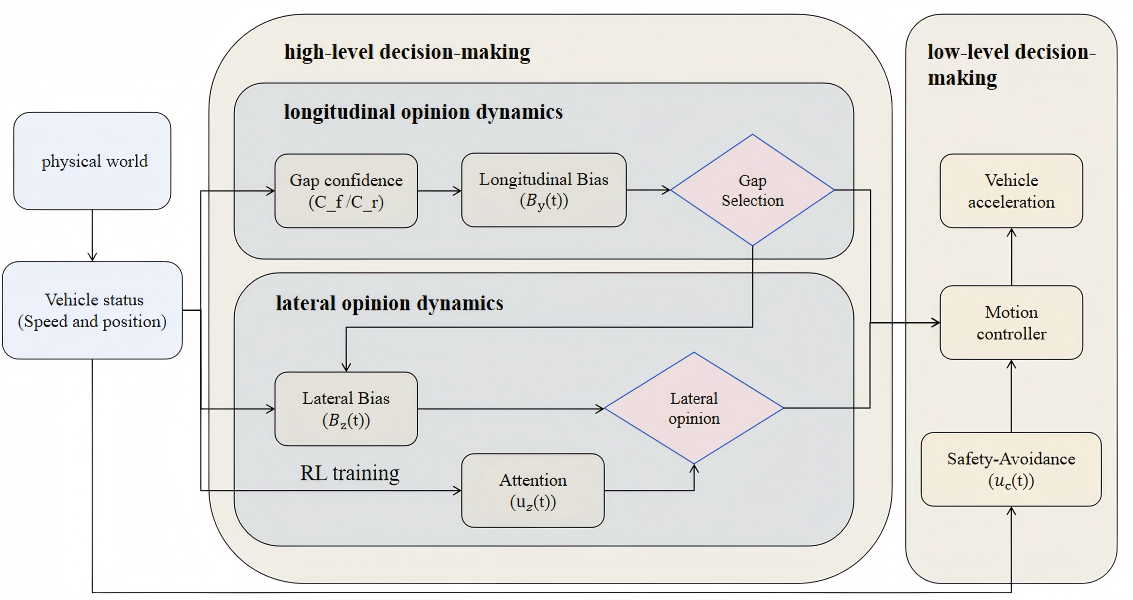
\includegraphics[width=0.60\linewidth]{System_block_diagram.png}
\caption{Control system structure block diagram}
\label{fig:system-block-diagram}
\end{figure}

\subsection{High-Level Decision-Making}

\subsubsection{Opinion Dynamics and Self-Update}

The same continuous opinion-dynamics template \cite{R16} is used for both high-level opinions. Let \(o(t)\in\mathbb{R}\) be a scalar opinion, \(u(t)\geq 0\) be its scalar attention intensity, \(b(t)\in\mathbb{R}\) be an external environmental bias, \(d>0\) be a damping coefficient, and \(\alpha>0\) be a sensitivity coefficient. The opinion evolves as

{\small
\begin{equation}
\dot{o}(t)=-d\,o(t)+u(t)\tanh\!\left(\alpha o(t)\right)+b(t).
\end{equation}
}

The damping term pulls the opinion toward neutrality, the hyperbolic-tangent term provides bounded self-reinforcement, and the bias term injects environmental evidence. A weak but persistent bias can therefore be amplified into a stable decision, while an unsupported opinion decays. For the longitudinal opinion, the scalar attention \(u_h(t)\) is updated by a Hill-type self-update law,

{\small
\begin{equation}
\dot{u}_h(t)=\frac{-u_h(t)+S_h(y(t)^2)}{\tau_h},\quad
S_h(y^2)=U_{\max}\frac{(y^2)^n}{K_h^n+(y^2)^n}.
\end{equation}
}

Here, \(\tau_h\) is the attention time constant, \(U_{\max}\) is the upper attention bound, \(K_h\) is the activation threshold, and \(n\) controls the steepness. Because \(S_h\) depends on \(y^2\), positive and negative directional opinions are reinforced symmetrically.

\subsubsection{Longitudinal Direction Bias Design}

At each time step, the high-level module selects the three target-lane vehicles closest to the ego front axle in the longitudinal coordinate. Let their scalar longitudinal positions be ordered from front to rear as \(x_{i_1}>x_{i_2}>x_{i_3}\). The forward candidate gap is formed by \((i_1,i_2)\), and the rear candidate gap is formed by \((i_2,i_3)\). For a candidate gap \(g\) with front vehicle \(F\) and rear vehicle \(R\), the scalar gap centre \(x_g(t)\) and scalar gap velocity \(v_g(t)\) are

{\small
\begin{equation}
x_g(t)=\frac{x_F(t)+x_R(t)}{2},\qquad
v_g(t)=\frac{v_F(t)+v_R(t)}{2}.
\end{equation}
}

Let \(x_e(t)\) and \(v_e(t)\) denote the ego front-axle longitudinal position and speed. The longitudinal alignment error is \(d_g(t)=x_g(t)-x_e(t)\), and the relative speed error is \(\Delta v_g(t)=v_g(t)-v_e(t)\). The confidence of candidate gap \(g\) is evaluated by a radial-basis function,

{\small
\begin{equation}
C_g(t)=
\exp\!\left(
-\frac{d_g(t)^2}{2\sigma_d^2}
-\frac{\Delta v_g(t)^2}{2\sigma_v^2}
\right),
\end{equation}
}

where \(\sigma_d\) and \(\sigma_v\) define the position and velocity bandwidths. If \(C_f(t)\) and \(C_r(t)\) are the confidences of the forward and rear candidate gaps, the longitudinal bias is \(B_y(t)=C_f(t)-C_r(t)\). This difference retains both direction and magnitude: \(B_y>0\) favours the forward gap, \(B_y<0\) favours the rear gap, and \(B_y\approx0\) indicates ambiguous evidence. Even a small confidence difference can become decisive when it persists, because the opinion dynamics amplifies temporally consistent evidence.

\subsubsection{Longitudinal Opinions and Decisions}

The longitudinal opinion \(y(t)\in\mathbb{R}\) accumulates the directional preference between the two candidate gaps. With the bias \(B_y(t)\) and attention \(u_h(t)\), its continuous dynamics are

{\small
\begin{equation}
\dot{y}(t)=-d_y y(t)+u_h(t)\tanh\!\left(\alpha_y y(t)\right)+B_y(t),
\end{equation}
}

where \(d_y\) and \(\alpha_y\) are the longitudinal damping and sensitivity coefficients. The selected gap is determined by a waiting band: the forward gap is selected when \(y(t)>\theta_y\), the rear gap is selected when \(y(t)<-\theta_y\), and no switch is made when \(|y(t)|\leq\theta_y\). This continuous formulation avoids an instantaneous max comparison and reduces frequent changes when the two candidate gaps have similar confidence.

\begin{figure}[!htbp]
\centering
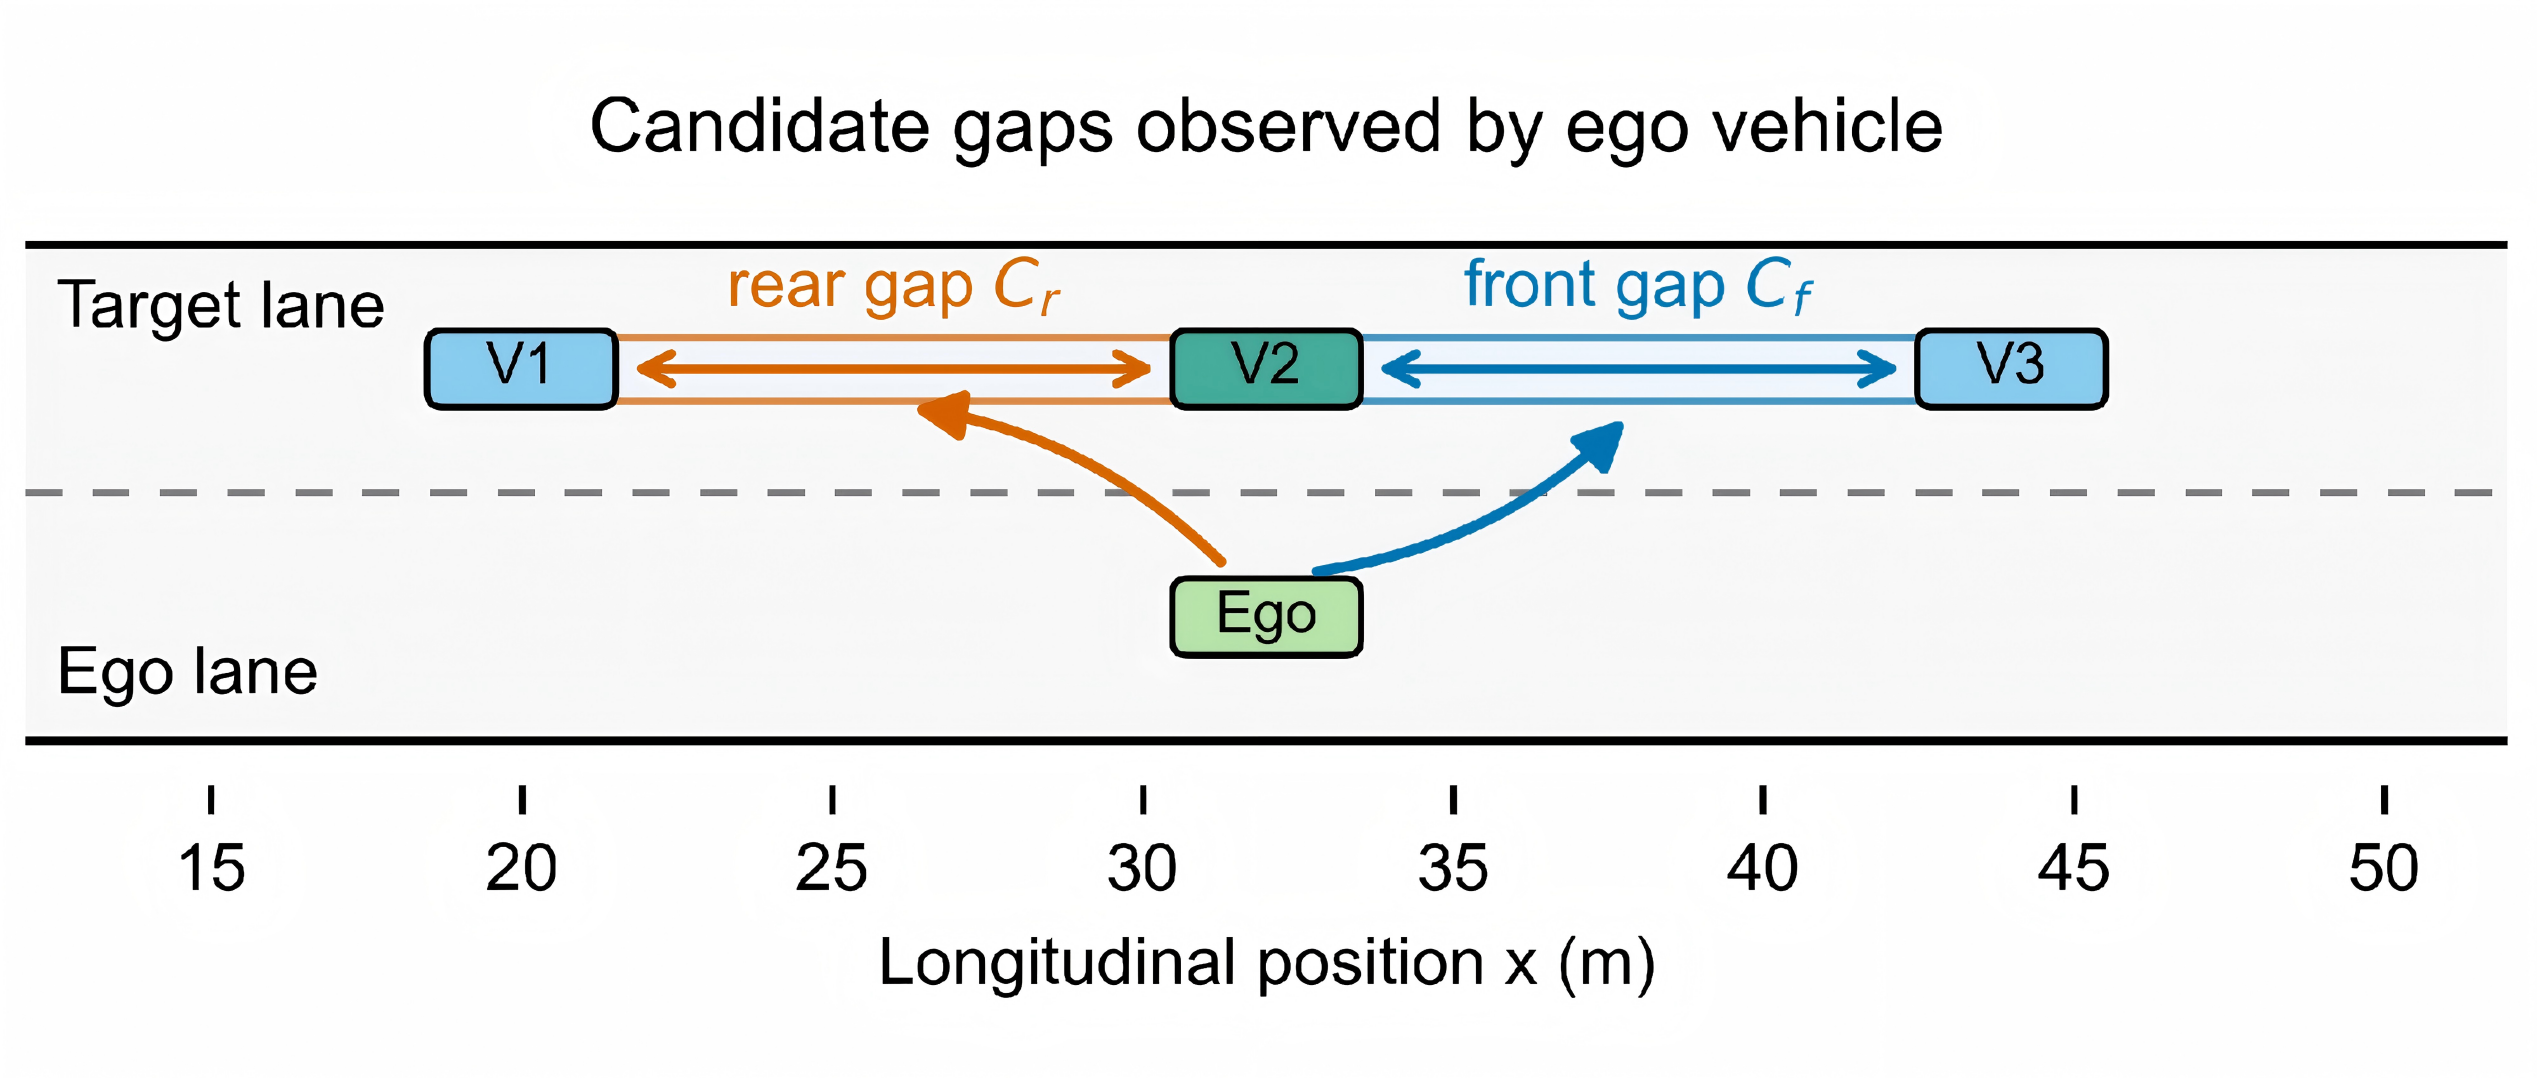
\includegraphics[width=0.60\linewidth]{layered_opinion_decision_schematic.png}
\caption{Layered opinion decision schematic}
\label{fig:layered-opinion-decision-schematic}
\end{figure}

\subsubsection{Lateral Direction Bias Design}

After the longitudinal decision chooses a target gap, the lateral opinion evaluates whether the ego vehicle should actively move toward it. For the selected front and rear vehicles, the scalar physical gap length is \(G(t)=x_F(t)-x_R(t)\), and the gap opening rate is \(\dot{G}(t)=v_F(t)-v_R(t)\). The lateral environmental bias is

{\small
\begin{equation}
B_z(t)=k_g\left[G(t)-G_{\mathrm{safe}}\right]+k_v\dot{G}(t),
\end{equation}
}

where \(G_{\mathrm{safe}}\) is the required safe gap, \(k_g\) weights the spatial margin, and \(k_v\) weights the rate of gap expansion. A large and opening gap increases \(B_z\), whereas a small or closing gap delays lateral commitment.

\subsubsection{Lateral Attention and SAC Design}

The lateral attention \(u_z(t)\) controls how strongly the lateral opinion self-reinforces. It is difficult to tune this attention manually because the system contains nonlinear opinion dynamics, moving traffic, collision penalties, and input limits. The Soft Actor-Critic (SAC) policy therefore outputs \(u_z(t)\) directly, while the model-based controller still determines the vehicle motion. Let \(s_t\) be the state, \(a_t\) be the action, \(\rho_\pi\) be the state-action distribution induced by policy \(\pi_\phi(a|s)\), \(r(s_t,a_t)\) be the immediate reward, \(\alpha_{\mathrm{SAC}}\) be the entropy temperature, and \(\mathcal{H}\) be policy entropy. SAC optimizes the policy by balancing return and entropy,

{\small
\begin{equation}
J(\pi)=\sum_t \mathbb{E}_{(s_t,a_t)\sim\rho_\pi}
\left[r(s_t,a_t)+\alpha_{\mathrm{SAC}}\mathcal{H}\!\left(\pi(\cdot|s_t)\right)\right].
\end{equation}
}

The state \(s_t\in\mathbb{R}^8\) contains the relative longitudinal and lateral positions and velocities between the ego vehicle and the front/rear vehicles of the selected gap. The action is the scalar attention command \(a_t=u_z(t)\), clipped to a fixed range:

{\small
\begin{equation}
s_t=[\Delta x_F,\Delta y_F,\Delta v_{x,F},\Delta v_{y,F},
\Delta x_R,\Delta y_R,\Delta v_{x,R},\Delta v_{y,R}],\qquad
a_t=u_z(t).
\end{equation}
}

The reward combines lane-change progress, opportunity usage, action smoothness, safety, and terminal success. The notation \(\mathbb{I}\{\cdot\}\) denotes an indicator function that equals one when its condition is true and zero otherwise:

{\small
\begin{equation}
\begin{aligned}
r_t={}&5\Delta p_t+2O_t\max(\Delta p_t,0)-0.02(1-p_t)
-0.5\|a_t-a_{t-1}\|^2 \\
&-2\mathbb{I}\{v_y(t)v_y(t-\Delta t)<0\}
-20\max\!\left(0,\frac{m_s-d_{\min}}{m_s}\right)^2 \\
&-1000\mathbb{I}\{\mathrm{collision}\}+(100-2t)\mathbb{I}\{\mathrm{success}\}.
\end{aligned}
\end{equation}
}

Here, \(p_t\) is the lane-change progress, \(O_t\) indicates whether a useful merging opportunity exists, \(m_s\) is the safety margin, and \(d_{\min}\) is the minimum distance to the neighbouring vehicles. This design rewards active merging progress while penalizing collision risk, oscillatory lateral motion, and unnecessarily long execution.

\subsubsection{Lateral Opinions and Decisions}

The lateral opinion \(z(t)\in\mathbb{R}\) accumulates the commitment to move toward the selected gap. Given the learned attention \(u_z(t)\) and the lateral bias \(B_z(t)\), the opinion follows

{\small
\begin{equation}
\dot{z}(t)=-d_z z(t)+u_z(t)\tanh\!\left(\alpha_z z(t)\right)+B_z(t),
\end{equation}
}

where \(d_z\) and \(\alpha_z\) are the lateral damping and sensitivity coefficients. The opinion is mapped to a merge ratio \(\lambda_z(t)=\mathrm{clip}((z(t)+1)/2,0,1)\). When \(z(t)\) is low, the desired point remains close to the original lane; as \(z(t)\) increases, the desired point moves toward the centre of the selected gap in the target lane.

\subsection{Low-Level Control Design}

\subsubsection{Safety-Avoidance Term}

The low-level controller uses the high-level target while adding a safety-avoidance term inspired by dissipative barrier feedback for embodied opinion-dynamics lane-merging control \cite{R17}. Let \(p_e(t)\in\mathbb{R}^2\) be the ego front-axle position, \(p_j(t)\in\mathbb{R}^2\) be the position of a neighbouring vehicle \(j\), \(r_j(t)=p_e(t)-p_j(t)\) be the relative position vector, and \(d_j(t)=\|r_j(t)\|\) be the Euclidean distance. Let \(R_c\) be the activation distance and \(k_c\) be the avoidance gain. The avoidance vector is

{\small
\begin{equation}
u_c(t)=\sum_j
\mathbb{I}\{d_j(t)<R_c\}\,
k_c\left(\frac{1}{d_j(t)}-\frac{1}{R_c}\right)
\frac{r_j(t)}{d_j(t)^3}.
\end{equation}
}

The term is zero outside the activation distance and grows rapidly when the ego vehicle approaches another vehicle.

\subsubsection{Target Point and Tracking Error}

The target point is interpolated between the original-lane reference and the selected target-lane gap. Let \(L_p\) be the preview distance, \(y_O\) be the original-lane centre, \(y_T\) be the target-lane centre, \(p_O(t)=[x_e(t)+L_p,\;y_O]^\top\) be the original-lane preview point, and \(p_G(t)=[x_g(t),\;y_T]^\top\) be the selected gap centre in the target lane. The opinion-weighted target is

{\small
\begin{equation}
p_{\mathrm{tar}}(t)=(1-\lambda_z(t))p_O(t)+\lambda_z(t)p_G(t)+u_c(t),
\qquad
e_p(t)=p_{\mathrm{tar}}(t)-p_e(t).
\end{equation}
}

The vector \(e_p(t)\) is the front-axle tracking error used by the physical controller.

\subsubsection{Final Physical Input Design}

The physical controller converts the target error into acceleration and steering-rate commands. Let \(\psi(t)\) be the ego heading. The longitudinal and lateral unit vectors are \(e_\parallel(t)=[\cos\psi(t),\sin\psi(t)]^\top\) and \(e_\perp(t)=[-\sin\psi(t),\cos\psi(t)]^\top\). Let \(v_{\mathrm{tar}}(t)\) be the target velocity, \(k_a\), \(k_x\), and \(k_\omega\) be tracking gains, \(a_{\min}\) and \(a_{\max}\) be acceleration limits, and \(\omega_{\min}\) and \(\omega_{\max}\) be steering-rate limits. The commanded acceleration \(a(t)\) and steering-rate command \(\omega(t)\) are

{\small
\begin{equation}
\begin{aligned}
a(t)&=\mathrm{clip}\!\left(k_a(v_{\mathrm{tar}}(t)-v_e(t))+k_x e_p(t)^\top e_\parallel(t),a_{\min},a_{\max}\right),\\
\omega(t)&=\mathrm{clip}\!\left(k_\omega e_p(t)^\top e_\perp(t),\omega_{\min},\omega_{\max}\right).
\end{aligned}
\end{equation}
}

This final stage is deliberately separated from the high-level opinions. The opinion variables decide which gap to use and how strongly to merge, while the low-level controller executes the motion subject to tracking and safety constraints.

\section{Experimental Design}





The experiments are organized from simple to complex. The single-gap environment isolates the lateral attention and merge-commitment problem: it tests whether RL can learn when to increase attention and commit to merging when the target gap is fixed. The multi-gap environment introduces longitudinal high-level decisions: when several dynamic gaps exist simultaneously, it tests whether the system can select an appropriate local gap, avoid excessive switching, and safely execute merging. The experimental parameters are listed in the appendix.



\subsection{Single-Gap Merging Experiment}





The single-gap environment contains one front vehicle, one rear vehicle, and one ego vehicle. The front and rear vehicles travel in the target lane, and their longitudinal separation defines the only available merging gap. The ego vehicle starts from the original lane and attempts to merge into this gap. The lane width is \(W=4.0\,\mathrm{m}\). The initial target-vehicle states are \(x_F(0)=30.0\,\mathrm{m}\), \(x_R(0)=15.0\,\mathrm{m}\), and \(v_F(0)=v_R(0)=15.0\,\mathrm{m/s}\).





The ego vehicle has the same initial longitudinal speed but a randomized longitudinal initial position, \(x_e(0)=20.0+\xi\), \(\xi\sim\mathcal{U}(-5.0,5.0)\), \(y_e(0)=2.0\,\mathrm{m}\), and \(v_e(0)=15.0\,\mathrm{m/s}\). This randomization makes the training and evaluation less dependent on one special initial alignment. It forces the policy to learn an attention schedule that works when the ego vehicle starts slightly ahead of or behind the gap center.





The rear vehicle is deliberately designed to create a staged merging opportunity. Before \(t_y=20.0\,\mathrm{s}\), it follows a sinusoidal law with period \(P_s=6.0\,\mathrm{s}\), velocity-amplitude parameter \(A_s=4.0\,\mathrm{m/s}\), angular frequency \(\omega_s=2\pi/P_s\), and front-rear gap \(g(t)=x_F(t)-x_R(t)\).



{\small
\begin{equation}
\begin{aligned}
\omega_s&=\frac{2\pi}{P_s},\qquad P_s=6.0\,\mathrm{s},\qquad A_s=4.0\,\mathrm{m/s},\\
a_R(t)&=A_s\omega_s\cos(\omega_s t),\\
v_R(t)&=v_R(0)+A_s\sin(\omega_s t),\\
x_R(t)&=x_R(0)+v_R(0)t+\frac{A_s}{\omega_s}\left[1-\cos(\omega_s t)\right],\\
g(t)&=x_F(t)-x_R(t)=15.0-\frac{A_s}{\omega_s}\left[1-\cos(\omega_s t)\right],\quad 0\leq t\leq20.0.
\end{aligned}
\end{equation}
}


After \(20.0\,\mathrm{s}\), the rear vehicle starts yielding by tracking a desired front-rear gap \(g_{\mathrm{yield}}=20.0\,\mathrm{m}\). The acceleration law uses proportional and damping gains \(0.35\) and \(1.1\), with acceleration clipped to \([-5.0,2.0]\,\mathrm{m/s^2}\). The rear-vehicle acceleration becomes:



{\small
\begin{equation}
\begin{aligned}
a_R(t)&=\mathrm{clip}\left(0.35\left[g(t)-20.0\right]-1.1\left[v_R(t)-v_F(t)\right],-5.0,2.0\right),\quad t>20.0,\\
\dot{g}(t)&=v_F(t)-v_R(t),\qquad \ddot{g}(t)=-a_R(t),\qquad t>20.0.
\end{aligned}
\end{equation}
}


This piecewise construction has a clear purpose. Before \(20.0\,\mathrm{s}\), the gap is not intentionally opened for the ego vehicle, so the policy should avoid premature aggressive merging. After \(20.0\,\mathrm{s}\), the rear vehicle creates a larger gap and the correct behavior is to increase attention \(u(t)\), allow the opinion \(z(t)\) to grow, and move the target point toward the target lane.





The SAC agent uses a Gaussian policy with two hidden layers of width \(256\), two Q networks, target Q networks, replay-buffer learning, and entropy regularization. The main training parameters are \(200\) episodes, replay-buffer size \(2.0\times10^5\), batch size \(256\), \(1000\) initial random steps, discount factor \(\gamma=0.99\), target-update rate \(\tau=0.005\), and learning rates \(3\times10^{-4}\) for the policy, Q networks, and entropy temperature. The subsequent value comparison uses the same reward as defined above so that the learned and hand-designed policies are judged by an identical metric. In the radial-basis-function baseline, \(u_{\mathrm{base}}\) is the base attention, \(u_{\mathrm{amp}}\) is the attention amplitude, and \(\sigma_d\) and \(\sigma_v\) are the same position and velocity bandwidths used for gap confidence. The baseline comparison evaluates the trained SAC attention against



{\small
\begin{equation}
u_{\mathrm{RBF}}(t)=
u_{\mathrm{base}}+
u_{\mathrm{amp}}
\exp
\left(
-\frac{d_g(t)^2}{2\sigma_d^2}
-\frac{\Delta v_g(t)^2}{2\sigma_v^2}
\right).
\end{equation}
}





The evaluation repeats the simulation \(100\) times with shared random ego initial positions. For each random seed, both policies face the same initial \(x_e(0)\) and the same target-vehicle trajectory. The comparison reports each episode reward and summarizes the mean and standard deviation across trials.



\subsection{Multi-Gap Merging Experiment}



\begin{figure}[!htbp]
\centering
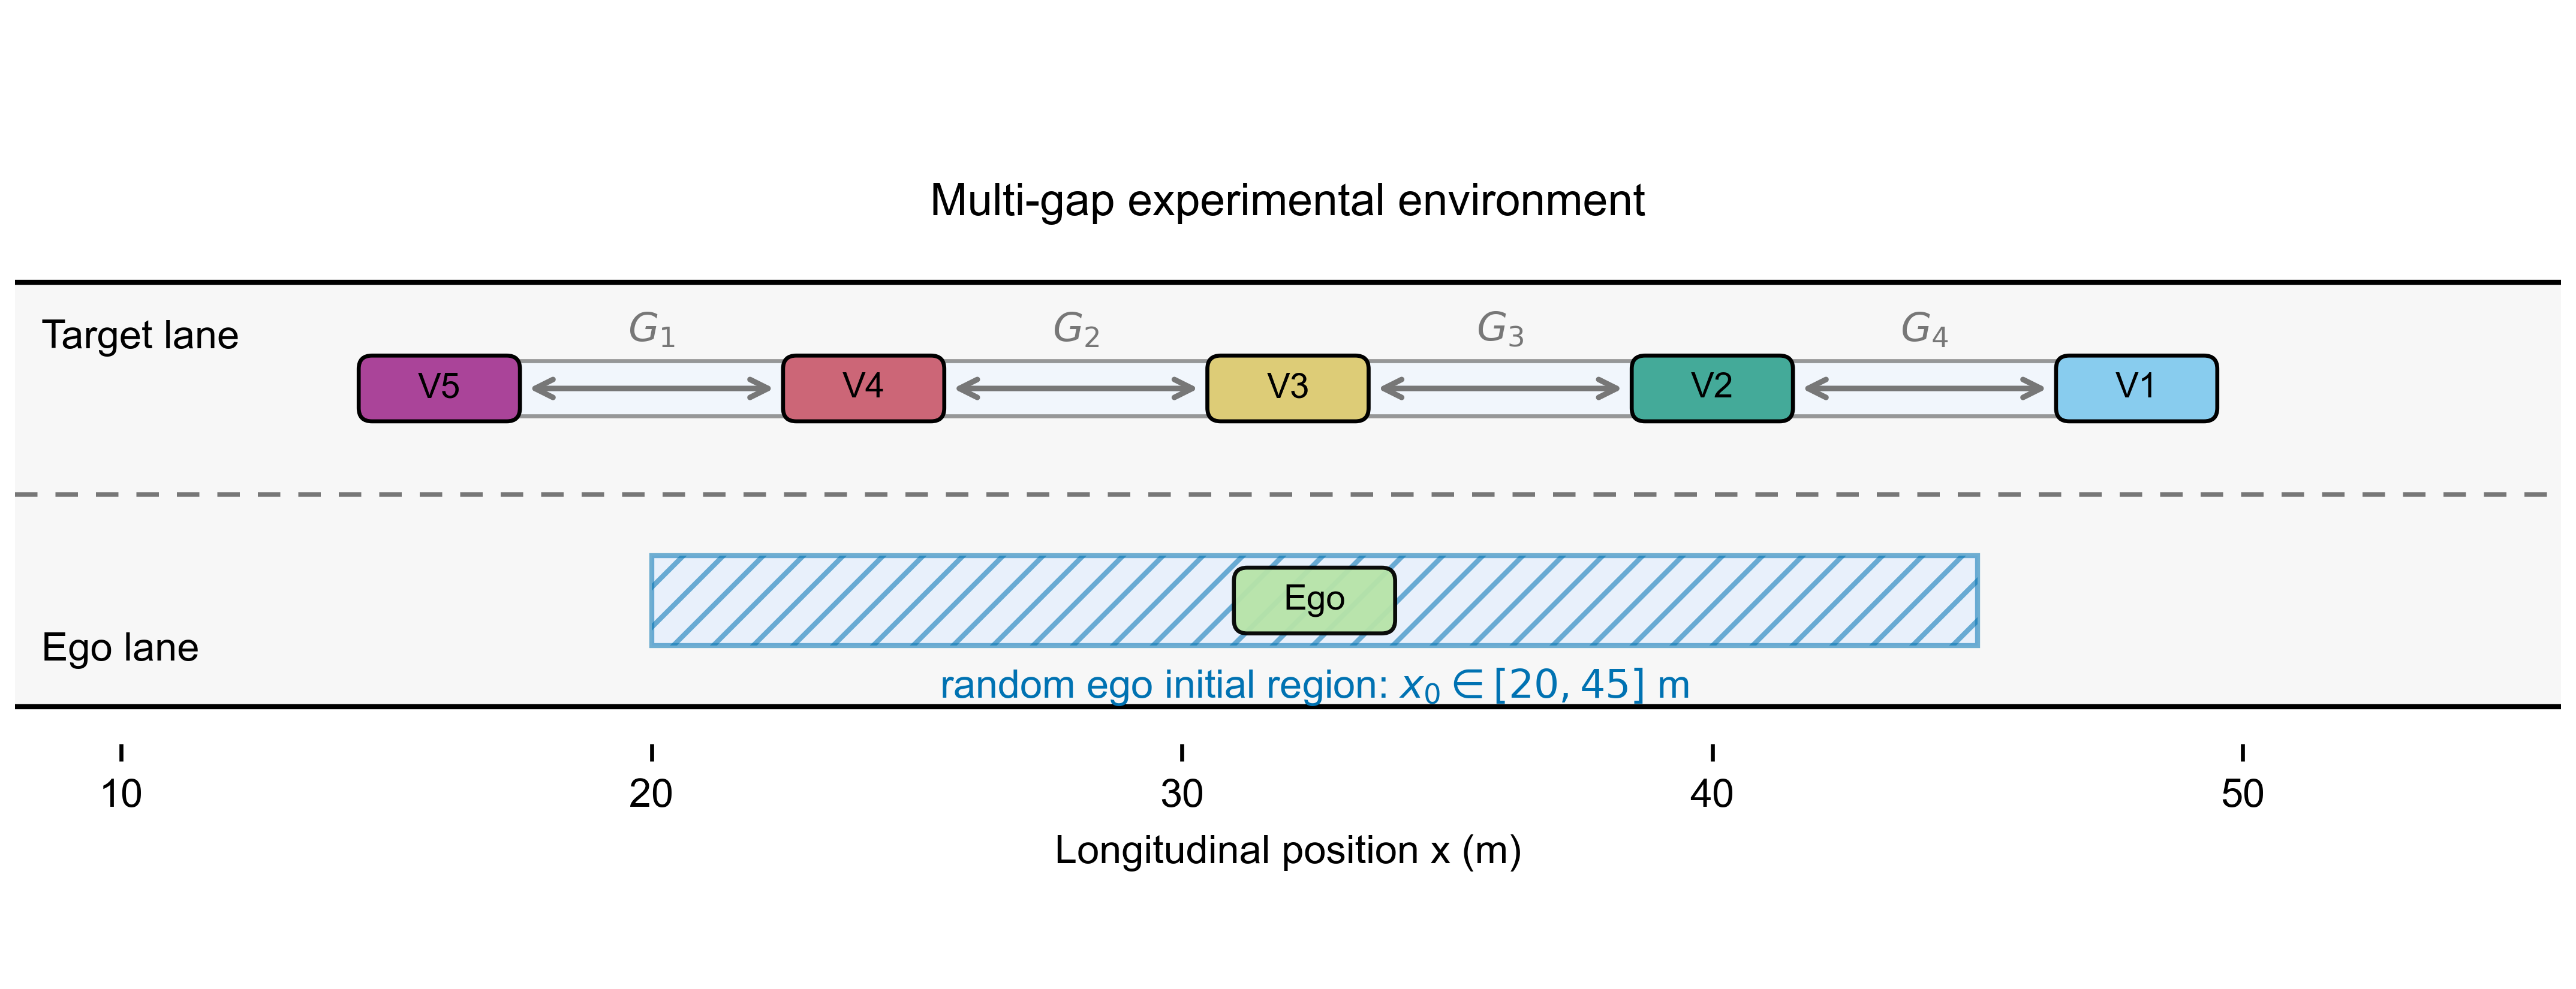
\includegraphics[width=0.60\linewidth]{multi_gap_environment_schematic.png}
\caption{multi gap environment schematic}
\label{fig:multi-gap-environment-schematic}
\end{figure}







The multi-gap environment extends the same merging task to a target lane containing five vehicles and four physical gaps. The target vehicles are initialized with a uniform base spacing, positions are \(x_i(0)=48.0-(i-1)g_0\), \(g_0=8.0\,\mathrm{m}\), \(i=1,\ldots,5\).





All target vehicles start on the target-lane center with nominal speed \(15.0\,\mathrm{m/s}\). The ego vehicle starts from the original lane with a larger longitudinal randomization range than in the single-gap experiment. The larger random range changes which three vehicles are nearest to the ego vehicle at the beginning of an episode. Therefore, the high-level selector must work under different local traffic configurations rather than repeatedly facing one fixed gap.





The ego initial state is \(x_e(0)=30.0+\xi\), \(\xi\sim\mathcal{U}(-10.0,15.0)\), \(y_e(0)=2.0\,\mathrm{m}\), and \(v_e(0)=15.0\,\mathrm{m/s}\).





The four target-lane gaps are randomly adjusted over time. Every \(T_g=4.0\,\mathrm{s}\), at most two gaps are selected for modification, and each selected gap receives a desired spacing from the multiplier set \(\mathcal{M}=\{0.75,1.0,1.25,1.5\}\).





The leading target vehicle has zero acceleration. For each following vehicle \(i+1\), let \(g_i(t)\) be its current gap to vehicle \(i\), \(g_{i,\mathrm{des}}^{(k)}\) be the desired gap during adjustment interval \(k\), and \(\dot{g}_i(t)\) be the gap-rate term. With proportional and damping gains \(0.55\) and \(1.05\), each following target vehicle tracks the desired gap through a clipped proportional-derivative rule:



{\small
\begin{equation}
a_{i+1}(t)=
\mathrm{clip}
\left(
0.55\left[g_i(t)-g_{i,\mathrm{des}}^{(k)}\right]
 +1.05\dot{g}_i(t),
-4.0,
4.0
\right).
\end{equation}
}





This mechanism produces a target lane in which gaps open, close, and reconfigure during the \(40.0\,\mathrm{s}\) simulation. The high-level decision module selects the nearest three target-lane vehicles in longitudinal front-axle coordinate and compares the two local gaps formed by these vehicles. The multi-gap experiment is designed to evaluate generalization. The underlying strategy uses the attention strategy learned in the single-gap environment. This design tests whether a strategy that only learns \(u(t)\) for a single pair of preceding and following vehicles remains effective when the high-level selector continuously provides different pairs of preceding and following vehicles. If the strategy is generalizable, then even if the gap selection and gap environment change, the ego vehicle should still be able to smoothly enter the selected gap.





The high-level ablation compares the opinion-dynamics selector with a simple maximum-score selector. The maximum-score baseline removes the high-level opinion memory and instantaneously chooses the candidate with the larger gap Confidence


This comparison was evaluated through multiple random ablation experiments. The current test setup uses \(N_{\mathrm{test}} = 100\) random runs. For each method, the total reward and the number of times the selected gap was switched were compared.



\section{Results and discussion}



\subsection{Single-gap SAC Training}



\begin{figure}[!htbp]
\centering
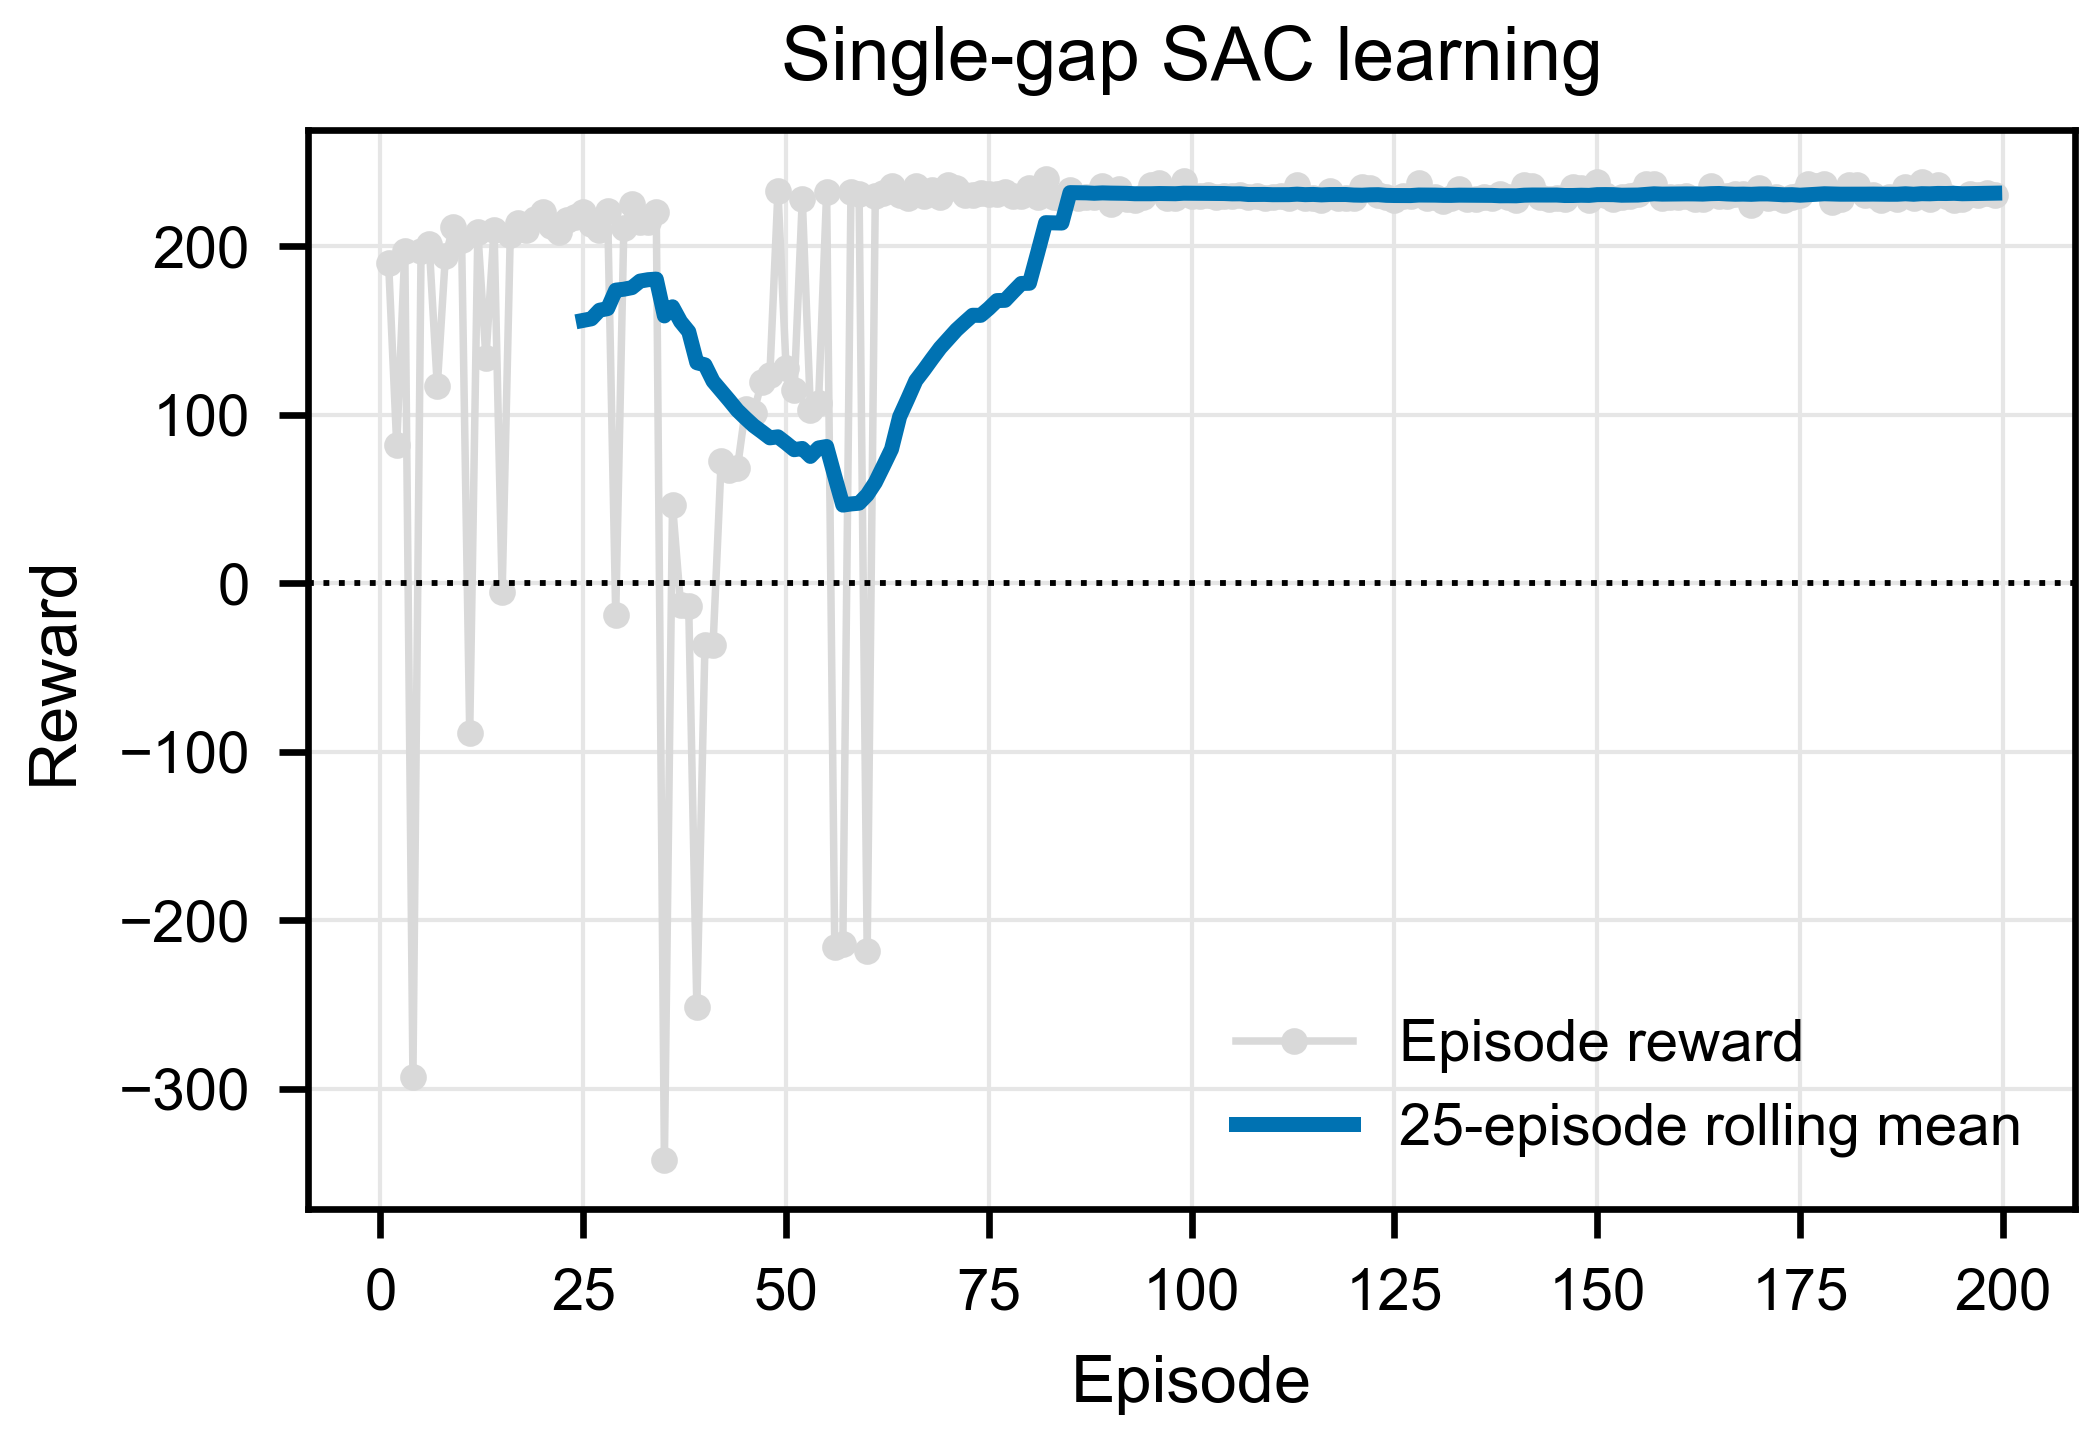
\includegraphics[width=0.60\linewidth]{fig1_single_gap_training.png}
\caption{single gap training reward}
\label{fig:fig1-single-gap-training}
\end{figure}







Training shows large reward fluctuations in the first 50 episodes because SAC explores widely. Afterward, the episodic reward stabilizes around 230\(\pm\)10 (Fig. 4). Q1-loss decreases from 134 to below 20, and the entropy coefficient \(\alpha\) decreases from 0.96 to 0.12. The final policy reaches progress \(\geq\) 0.95, achieves 97.5\% success, and produces no collisions.



\subsection{Comparison with Baseline RBF Controller}



\begin{figure}[!htbp]
\centering
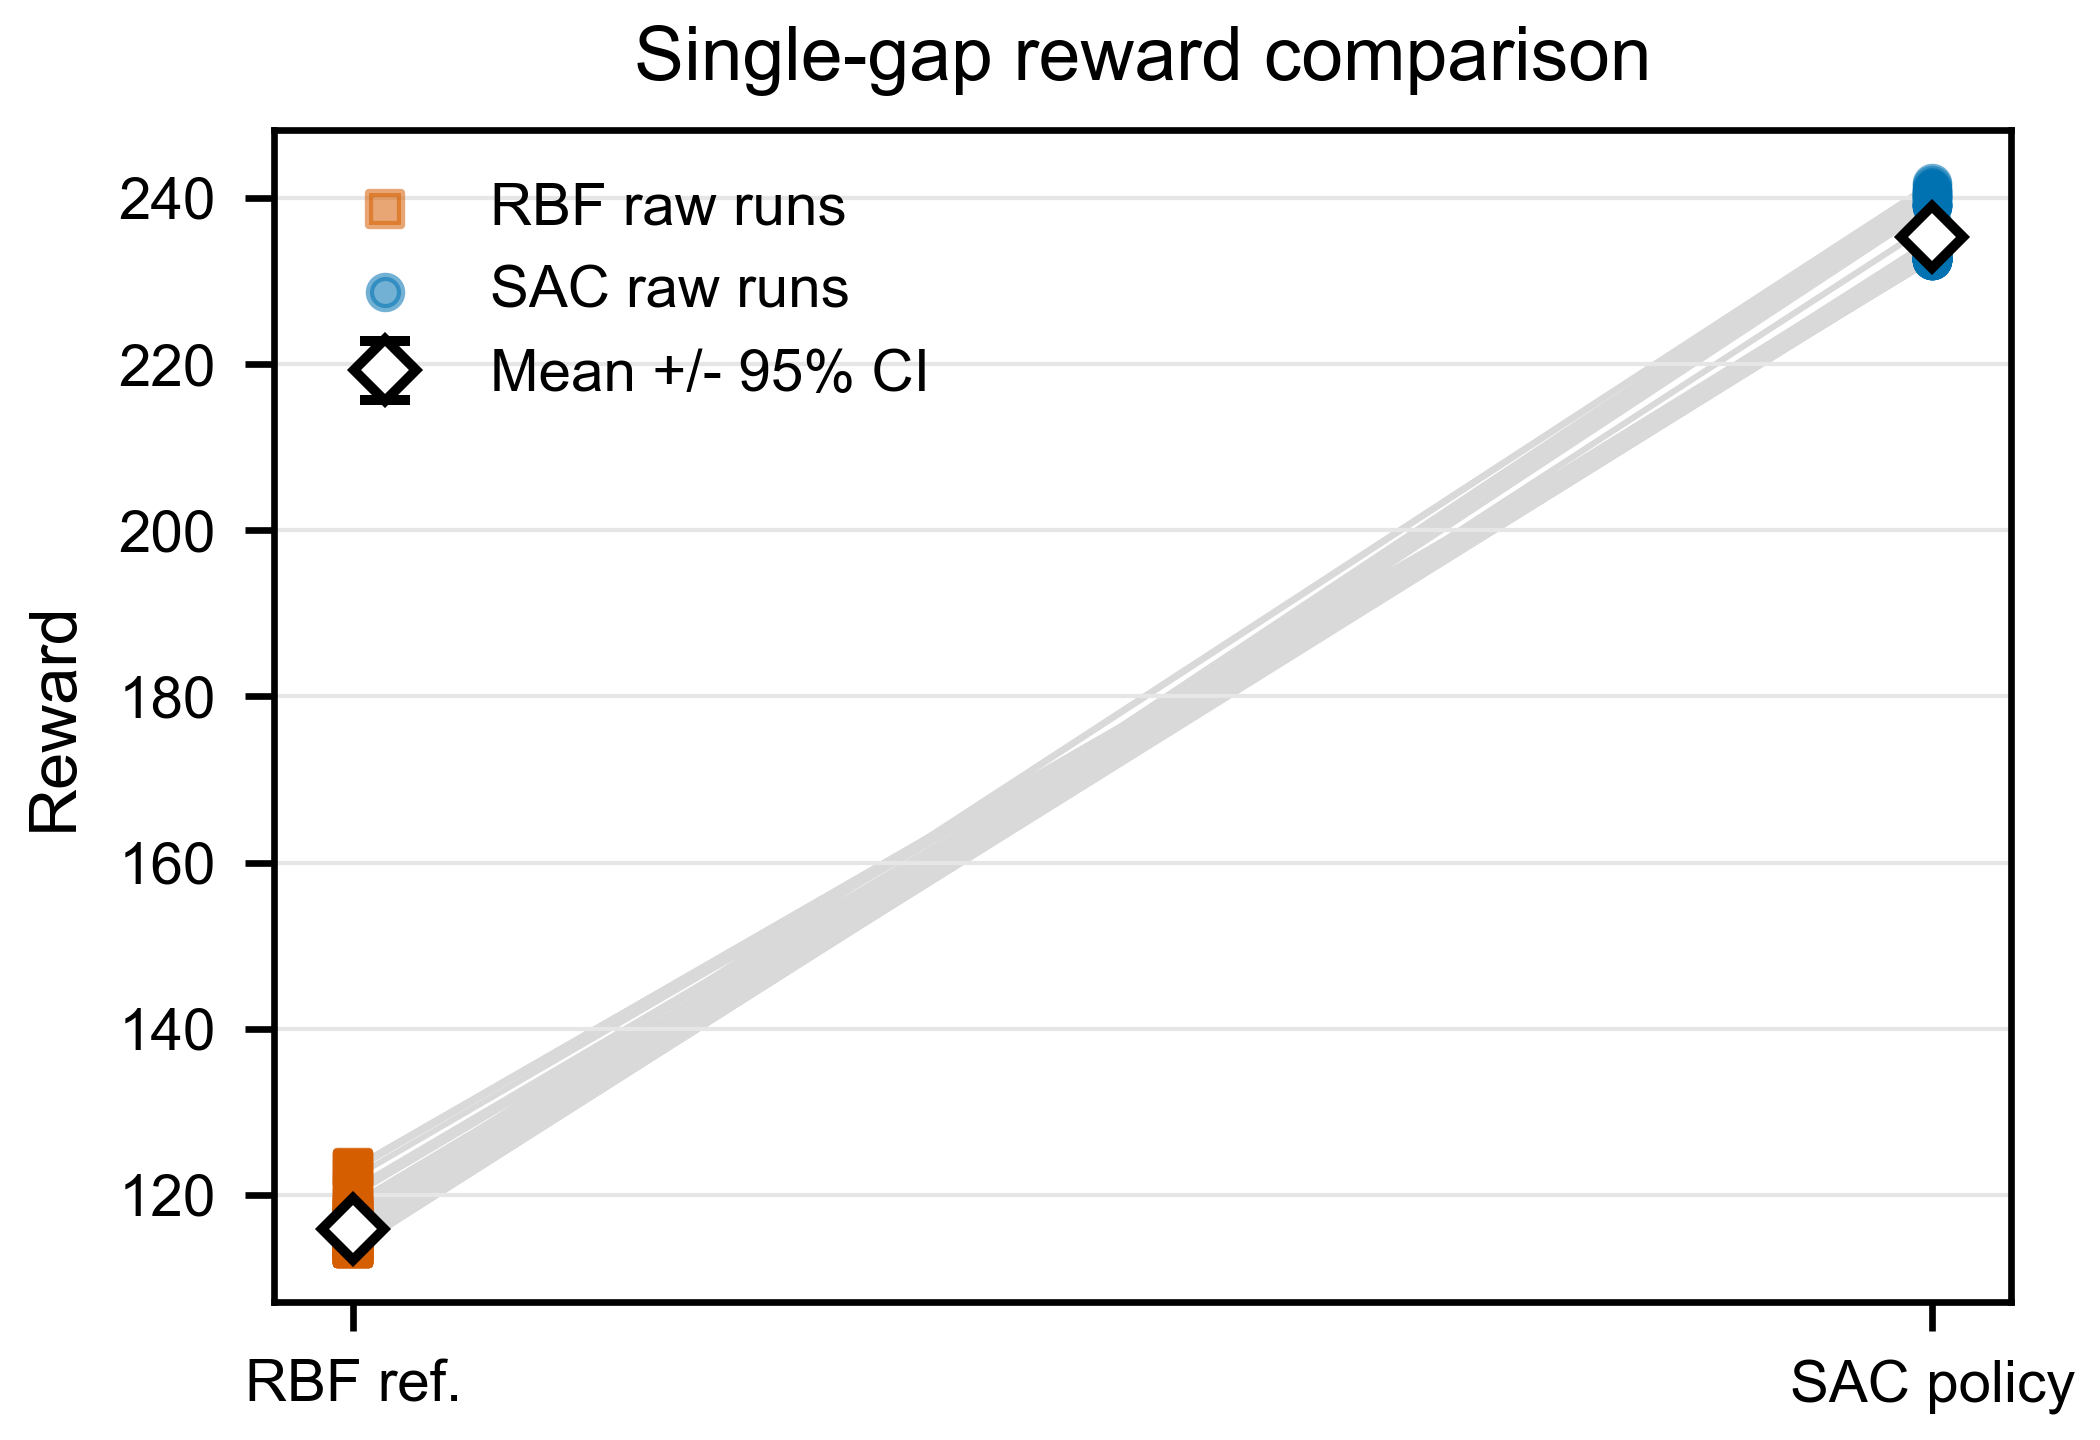
\includegraphics[width=0.60\linewidth]{fig2_single_gap_policy_vs_rbf.png}
\caption{Comparison between SAC and RBF reward}
\label{fig:fig2-single-gap-policy-vs-rbf}
\end{figure}







The SAC policy achieves a higher average episodic reward than the RBF baseline, with 233.4 versus 115.8. Both policies maintain 100\% success and zero collisions, but SAC completes the task in 6.9 s, whereas RBF requires 29.45 s. This indicates that the hand-designed RBF rule is safe but conservative, while SAC learns a more efficient yet still collision-free strategy.



In terms of safety indicators, the RBF baseline maintained a larger minimum distance ($d_{\min} \approx 9.7$ m), reflecting its inherent conservatism. The SAC attention policy is closer to the obstacle ($d_{\min} \approx 2.6$ m), but always remains outside the collision radius, showing that the learned attention can balance time efficiency and collision safety through the reward structure.



\begin{table}[!htbp]
\centering
\caption{Single-gap evaluation comparison between SAC and RBF controllers}
\label{tab:single-gap-policy-comparison}
\footnotesize
\begin{tabular}{p{0.23\linewidth}p{0.23\linewidth}p{0.23\linewidth}p{0.23\linewidth}}
\toprule
Metric & SAC Policy & RBF Baseline & Improvement \\
\midrule
\textbf{Episodic Reward} ($\bar{R}$) & \textbf{$233.4 \pm 4.2$} & $115.8 \pm 2.1$ & \textbf{+101.5\%} \\
\textbf{Task Time (s)} & \textbf{$6.9 \pm 0.2$} & $29.45 \pm 2.4$ & \textbf{-76.6\%} \\
\textbf{Success Rate} & 100\% & 100\% & N/A\\
\textbf{Collision Rate} & 0\% & 0\% & N/A\\
\textbf{Min. Distance (m)} & $2.62 \pm 0.23$ & $9.70 \pm 0.01$ & N/A\\
\bottomrule
\end{tabular}
\end{table}



\subsection{Multi-Gap Generalization}



\begin{figure}[!htbp]
\centering
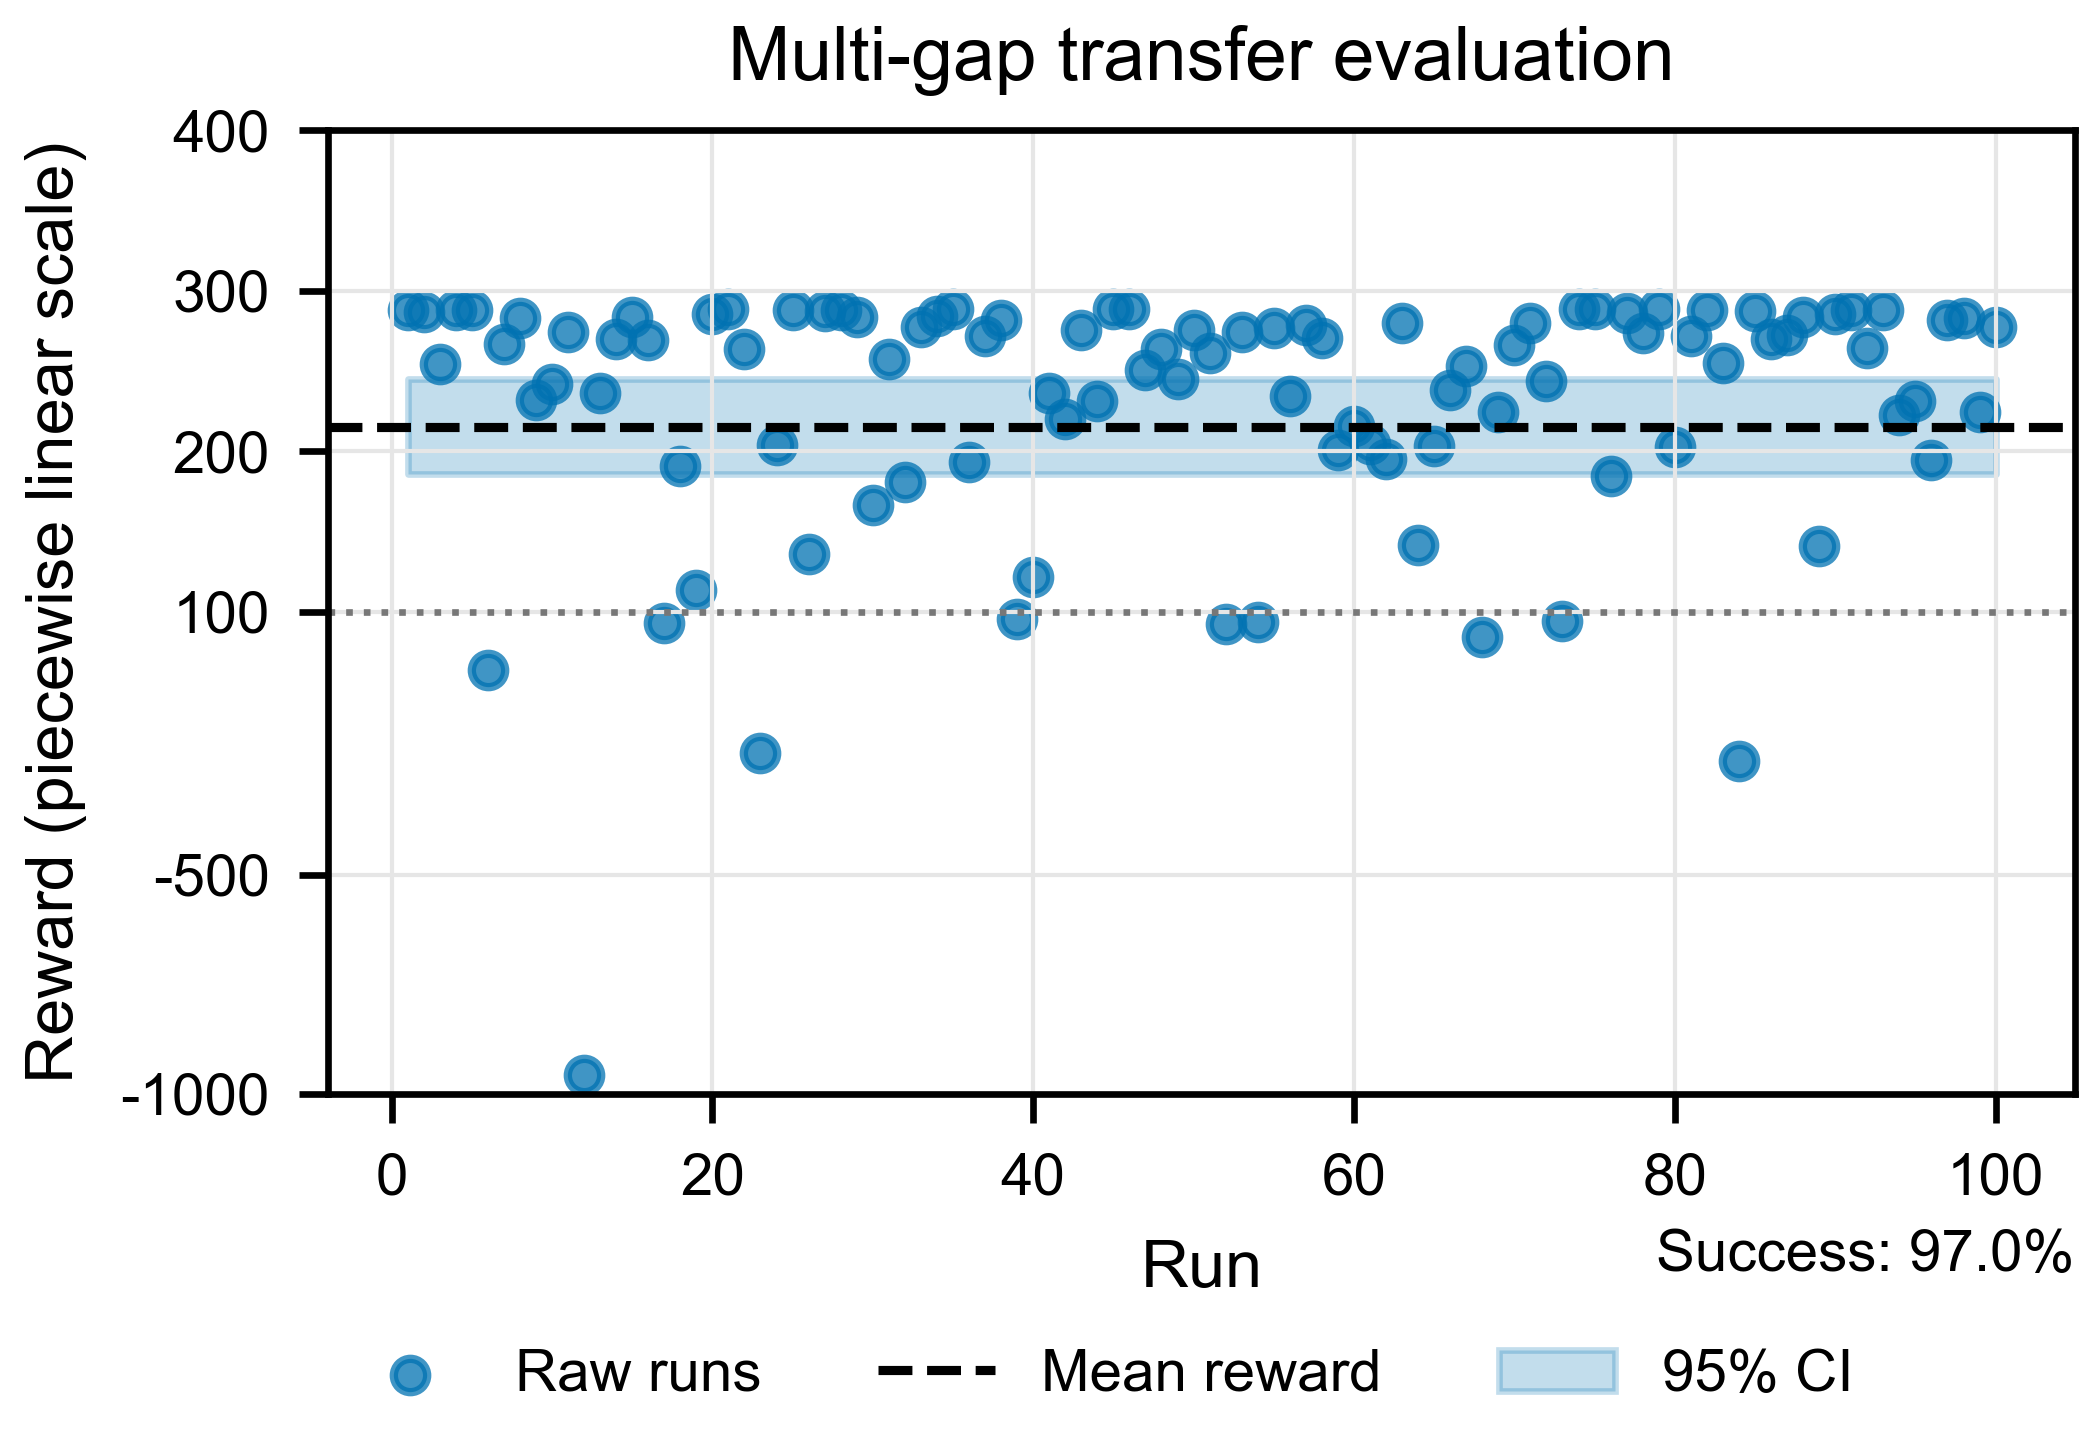
\includegraphics[width=0.60\linewidth]{fig3_multi_gap_transfer.png}
\caption{The reward of the multiple gap generalization experiments}
\label{fig:fig3-multi-gap-transfer}
\end{figure}







The lateral SAC attention policy was trained in a single-gap environment and then directly deployed to a dynamic multi-gap scenario. The experimental results show that it has good generalization ability in terms of safety and task completion: the success rate remains at a high level (\(\approx\)0.97). Even if the high-level selector switches, in the vast majority of cases, the lateral attention policy never violates the safety boundary. These data confirm that the learned attention policy generalizes beyond the training environment.



Some difficult cases still produce low reward or failure. These cases mainly arise from repeated high-level decisions that extend the manoeuvre beyond the maximum simulation time, or from overly cautious local optima that accumulate large step penalties. This suggests that the current state input is too instantaneous: it captures relative geometry and velocity but does not fully represent temporal gap switching or long-term feasibility.



\subsection{High-level decision-making Ablation experiment}



\begin{figure}[!htbp]
\centering
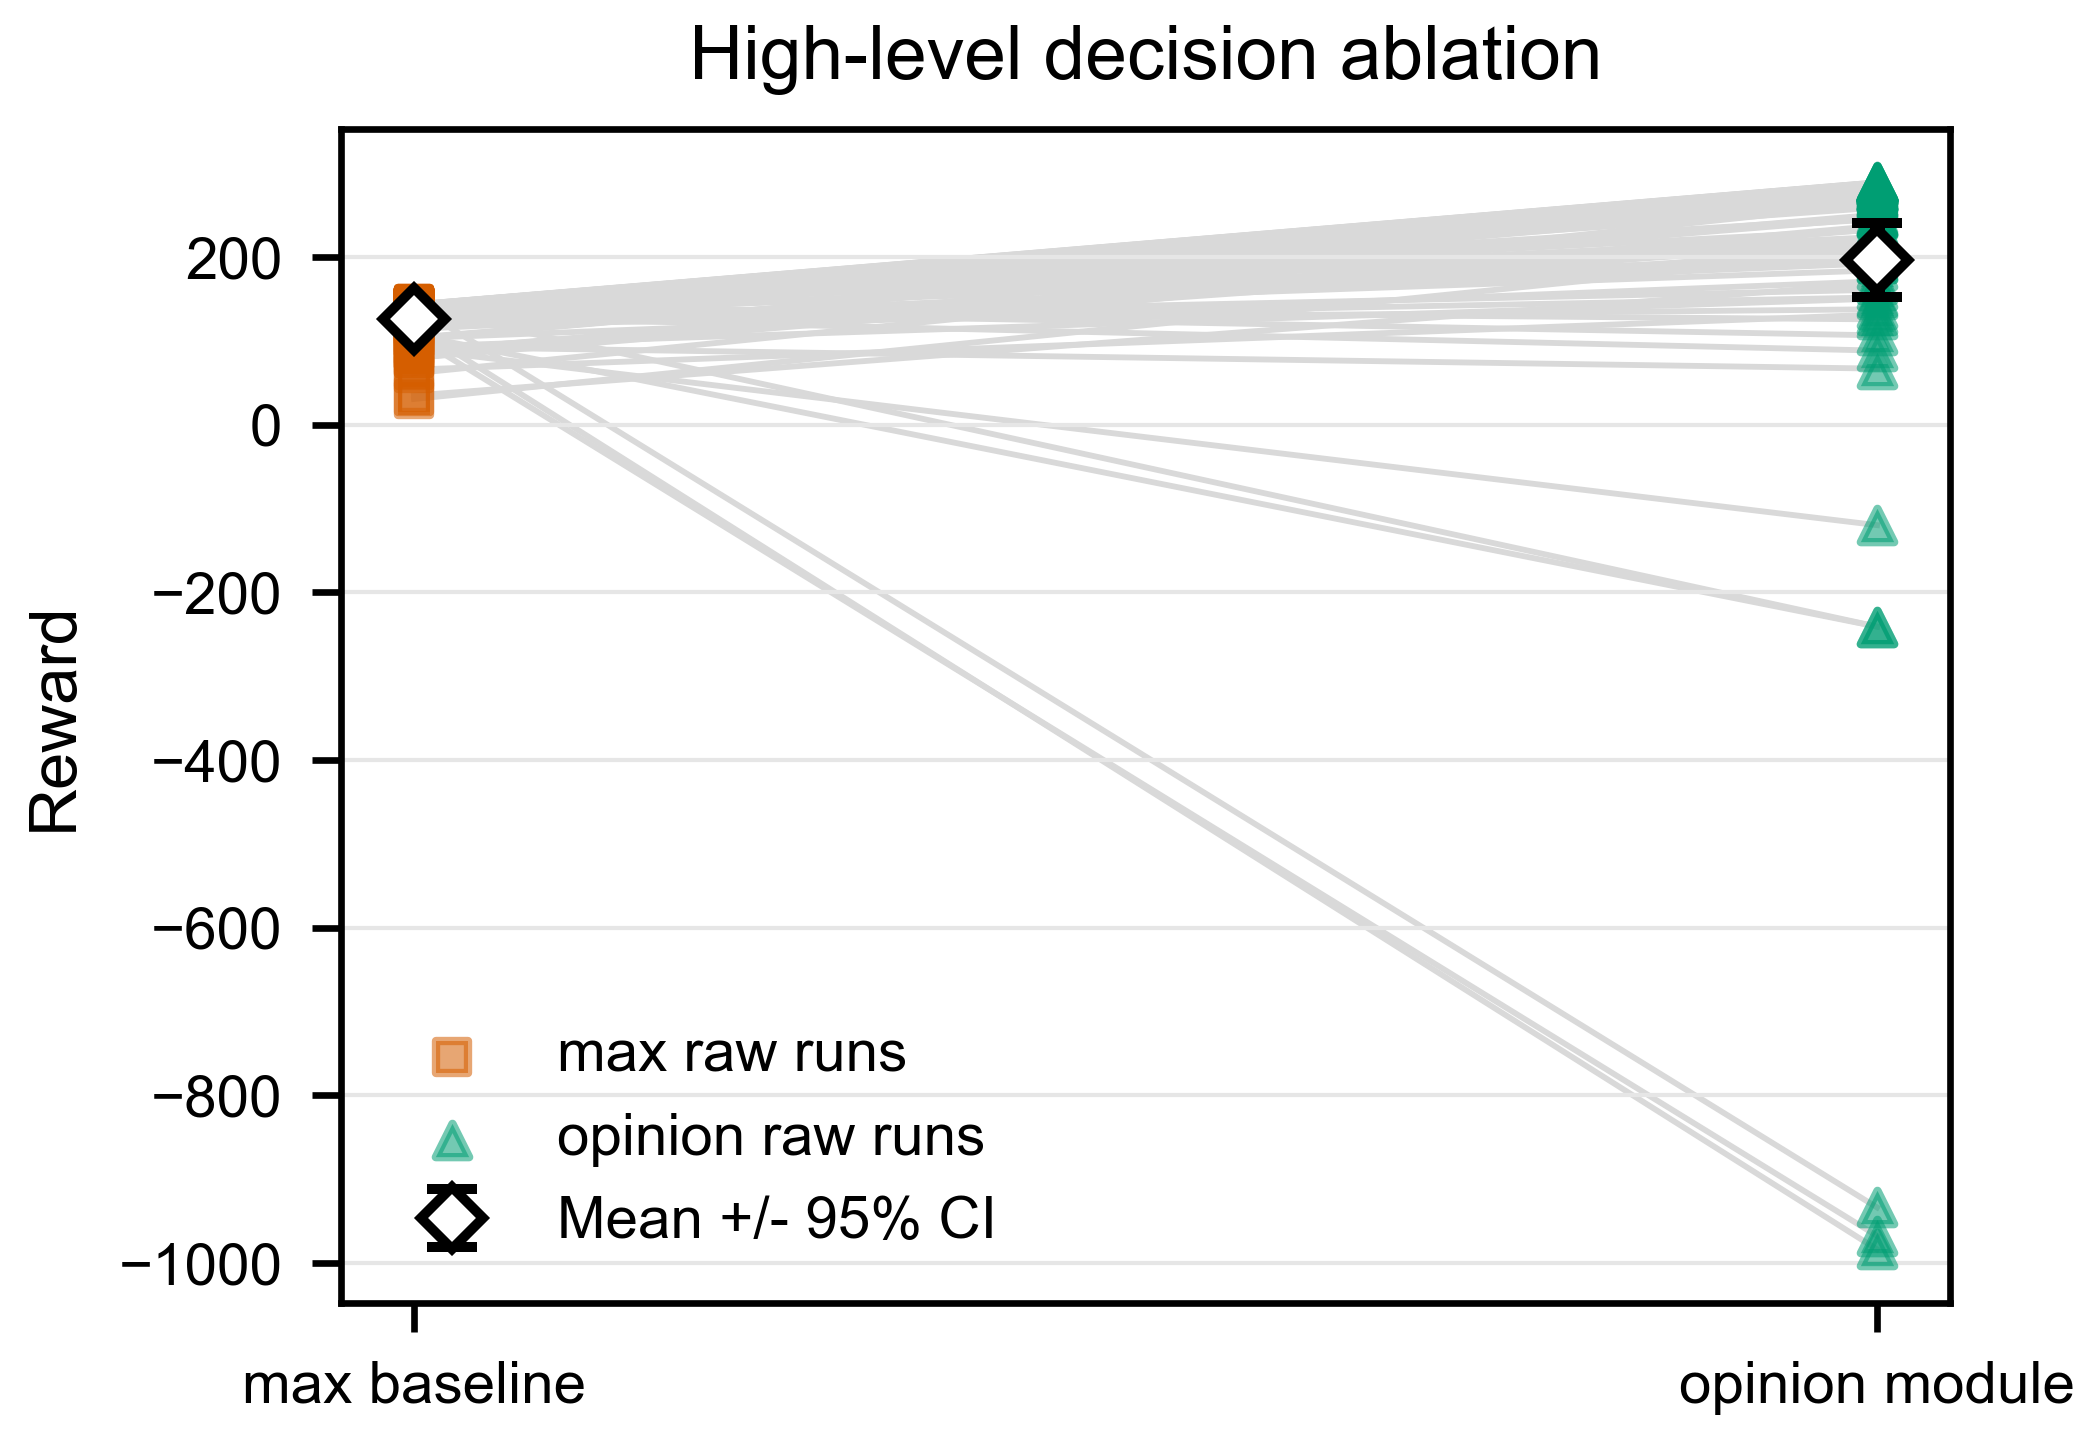
\includegraphics[width=0.60\linewidth]{fig4_multi_gap_ablation.png}
\caption{Comparison of high-level strategy rewards between Opinion and Max}
\label{fig:fig4-multi-gap-ablation}
\end{figure}







The opinion-dynamics selector achieves a higher mean reward than the max-score selector (+55.3\%) and switches less often (0.61 versus 0.76). Although max-score sometimes finishes faster, its lower reward indicates larger safety penalties and less smooth control. The opinion-based selector therefore provides more temporally consistent guidance and more stable behaviour, despite a slightly lower success rate caused by timeout cases.



\begin{table}[!htbp]
\centering
\caption{Multi-gap high-level decision ablation results}
\label{tab:multi-gap-ablation}
\footnotesize
\begin{tabular}{p{0.23\linewidth}p{0.23\linewidth}p{0.23\linewidth}p{0.23\linewidth}}
\toprule
Metric & Opinion Strategy & Max Strategy & Improvement \\
\midrule
\textbf{Mean Episode Reward} (\(\bar{R}\)) & $196.8 \pm 48.9$ & $126.7 \pm 28.7$ & \textbf{+55.3\%} \\
\textbf{Mean Switch Count} & $0.61 \pm 0.48$ & $0.76 \pm 0.79$ & \textbf{-19.7\%} \\
\textbf{Mean Time (s)} & 12.6 & 8.2 & N/A\\
\textbf{Success Rate} & \textbf{97\%} & 100\% & N/A\\
\bottomrule
\end{tabular}
\end{table}



\section{Conclusions}

The proposed two-layer framework provides an interpretable method for autonomous lane merging. The high-level decision-making layer uses longitudinal opinion dynamics to select a local candidate gap and lateral opinion dynamics to decide the strength of merging commitment. The low-level control layer then converts this high-level decision into collision-aware target tracking and physical vehicle inputs. This revised structure separates strategic decision formation from execution, while preserving a continuous opinion-dynamics formulation throughout the system.

Experiments show that the SAC-trained lateral attention policy in the single-gap environment converges to a stable behaviour and outperforms the hand-designed RBF attention baseline, mainly by reducing completion time while remaining collision-free. In the multi-gap environment, the same policy maintains a high success rate, indicating that the learned attention has partial generalization beyond the training scenario. The remaining failures mainly occur in difficult cases with repeated gap switching or excessive waiting, which suggests that future work should include temporal state information and stronger communication between longitudinal selection and lateral commitment. The ablation study further shows that the opinion-based high-level selector achieves higher reward and fewer switches than the max-score selector, confirming the value of temporally smoothed opinion dynamics for interactive lane-changing decisions.

\clearpage
\printbibliography[title={References},heading=bibintoc]

% BEGIN GENERATED DOCX APPENDICES

\begin{uomappendix}

\section{Project Outline}

Learning Decision Dynamics for Multi-Robot Teams: Hierarchical Strategy and Control

Project Scope

This research project is fundamentally situated at the intersection of multi-agent systems, nonlinear control theory, and machine learning. The primary scope encompasses the design, mathematical formulation, software implementation, and extensive simulation-based evaluation of a novel hierarchical framework. Specifically, the project will focus on employing Reinforcement Learning (RL) techniques to dynamically optimize the governing parameters of a nonlinear control system, which dictates the strategic opinion dynamics and physical behavior of a multi-robot team. The scope includes establishing a robust simulation environment (e.g., using ROS and Python) to model complex, interactive scenarios where robots must navigate the trade-offs between cooperative consensus and competitive dissensus. The boundary of this project is strictly confined to computational modeling and algorithmic simulation; it explicitly excludes any hardware deployment, physical robot trials, real-world outdoor testing, or human-in-the-loop experiments. All datasets generated and utilized will be purely synthetic.

Motivation

The deployment of multi-robot teams in highly dynamic and unpredictable environments---such as autonomous driving, search and rescue operations, and automated logistics---presents a formidable challenge. Traditional control strategies often rely on fixed, pre-computed parameters for their nonlinear dynamics models. While these deterministic approaches work well in static scenarios, they critically lack the flexibility needed when the environment rapidly shifts, or when the team needs to fluidly transition between cooperative and competitive behaviors. Furthermore, there is often a distinct disconnect between high-level strategic decision-making (e.g., task allocation) and low-level physical control (e.g., collision avoidance). By introducing state-of-the-art Reinforcement Learning methods to continuously and adaptively optimize the parameters of the nonlinear control systems, this project aims to bridge that critical gap. The motivation is to endow the robotic team with the "intelligence" to learn optimal decision dynamics directly from experiential feedback, thereby significantly enhancing the system's overall efficiency, safety, and adaptability in complex, multi-agent interactions.

Aim

Aim: The overarching aim of this research project is to develop, integrate, and extensively validate a comprehensive, hierarchical decision-making and control framework for multi-robot systems. This framework will leverage Reinforcement Learning algorithms to intelligently tune the parameters of a nonlinear control system, enabling distributed agents to reach rapid strategic consensus or dissensus while strictly adhering to safety-critical physical constraints in a fully simulated, highly dynamic environment.

Objectives

To realize the overarching aim, this project is broken down into the following specific, measurable objectives:

Mathematical Formulation: To construct a rigorous strategic-level mathematical model utilizing nonlinear opinion dynamics that dictates distributed consensus, role assignments, and task allocation among the multi-robot team.

RL-Based Parameter Optimization: To design and train a Reinforcement Learning agent (e.g., utilizing algorithms such as Proximal Policy Optimization or Soft Actor-Critic) dedicated to dynamically optimizing the critical tuning parameters of the nonlinear control system, allowing the team's cooperative/competitive behavior to adapt in real-time to environmental stimuli.

Safe Control Execution: To develop an execution-level control strategy (incorporating methods like Control Barrier Functions) that securely translates high-level strategic objectives into collision-free kinodynamic trajectories, ensuring that physical constraints are never violated.

System Integration: To seamlessly integrate the high-level RL-driven decision dynamics with the low-level safety controllers within a robust, multi-agent simulation framework (e.g., using ROS 2 and Python-based physics engines).

Performance Evaluation: To conduct exhaustive simulation trials across varied operational scenarios, benchmarking the RL-optimized system against traditional fixed-parameter baseline controllers by evaluating metrics such as convergence speed, safety violation rates, and overall task efficiency.

\section{Risk Assessment}

General Risk Assessment Form

{\small
\begin{description}
\item[Date:] 2026.7.1.
\item[Assessed by:] Junyi Lei.
\item[Checked / Validated by:] .
\item[Location:] Home.
\item[Assessment ref no:] .
\item[Review date:] .
\item[Task / premises:] Software development, algorithm simulation (RL for nonlinear control), data analysis, and report writing.
\end{description}

\subsection*{Risk Items}

\begin{itemize}[leftmargin=*]
\item \textbf{Working from home: Lone working.} Hazard: lone working. Who might be harmed and how: home working staff may become isolated. Existing measures: refer to the University Lone Working policy and guidance, the University Working at Home guidance, and the University Wellbeing Support website. Staff are able to have regular direct contact with line managers and colleagues via phone, Teams, Zoom, or email. Risk rating: Low. Result: A.

\item \textbf{Working from home: Poor posture, repetitive movements, and eye strain from long periods looking at DSE.} Who might be harmed and how: staff, students, and visitors may experience back strain due to poor posture, repetitive strain injury to upper limbs, and eye strain. Existing measures: refer to the DSE policy, guidance, and poster for workstation setup; complete the DSE self-assessment for home working at least every two years or sooner if changes or pain are experienced; complete the homeworking self-assessment checklist; set up the workstation in a comfortable position with good lighting and natural light where possible; take regular breaks away from the screen; regularly stretch arms, back, neck, wrists, and hands; use a desktop working space where possible and avoid working on a laptop without a docking station, separate keyboard, or mouse; small equipment purchases of up to GBP 50 may assist with working from home; contact local administration for more details; if ill-health issues occur, contact the local DSE assessor or safety advisor for a full DSE assessment; occupational health referral may be used where issues cannot be resolved; DSE users should have regular eye tests and follow FSE guidance. Risk rating: Low. Result: A.

\item \textbf{Working from home: Stress / wellbeing.} Who might be harmed and how: home working staff may experience psychosocial effects, work-life imbalance, anxiety, poor performance, fatigue, and tiredness. Existing measures: refer to the Stress Prevention and Management toolkit, University guidance for managing teams working from home, AMBS Seven Rules of Home Working, and guidance for managers and staff; complete Work Related Stress: Identification, Prevention and Management training; use the University Stress Assessment tool where appropriate; discuss projects, work plans, and objectives with the line manager regularly; maintain regular contact meetings with managers and peers via Teams, Zoom, email, and phone; define working hours and daily routines; prioritise tasks; individuals may self-refer to Occupational Health Service or to the Counselling and Mental Health Service. Risk rating: Low. Result: A.

\item \textbf{Use of electrical appliances.} Hazard: misuse of electrical appliance or faulted electrical appliance. Who might be harmed and how: home working staff may face electric shock, burns, and fire. Existing measures: use all office equipment according to manufacturer instructions; make visual checks before use to ensure equipment and cables are free from defects; University IT equipment brought home should already be PAT tested; small electrical items can be tested through the FSE I\&F team; domestic electrical supply and employee-owned equipment are the employee's responsibility to maintain; clean liquid spills immediately; defective plugs, cables, and equipment should be taken out of use. Risk rating: Med. Result: A.

\item \textbf{Moving around the home office.} Hazard: obstructions and trip hazards. Who might be harmed and how: home working staff may suffer slips, trips, and falls causing physical injury. Existing measures: keep floors and walkways clear of items such as boxes, packaging, and equipment; arrange furniture so movement of people and equipment is not restricted; ensure good lighting; maintain reasonable housekeeping; position trailing cables neatly away from walkways; keep cabinet drawers and doors closed when not in use. Risk rating: Med. Result: A.

\item \textbf{Working from home: Fire.} Who might be harmed and how: staff home working may face risk of burns, smoke inhalation, and asphyxiation. Existing measures: in the event of fire, evacuate the building and call the fire brigade on 999; remove all combustible waste regularly; locate heaters away from combustible materials and switch them off when not in use; do not leave heaters unattended; avoid daisy chaining and overloading extension leads; test smoke alarms routinely and replace batteries every 6--12 months; refer to fire brigade Home Fire Safety and Smoke Alarms. Risk rating: Med. Result: A.
\end{itemize}

\subsection*{Action Plan}

\begin{enumerate}[leftmargin=*]
\item DSE Self-Assessment: Complete the workstation self-assessment to prevent physical strain (neck/back/eyes) during extended ROS 2 programming and RL training sessions. Action by: Student. Action by when: Week1. Done: .
\item Workload \& Stress Management: Implement regular timeline reviews with the supervisor to manage stress, ensuring the project milestones and dissertation writing remain on track for the final September submission deadline. Action by: Student. Action by when: Week2-3. Done: .
\item Data Backup: Establish automated version control and secure backups for simulation logs, RL models, and draft reports to prevent data loss due to computer failure. Action by: Student. Action by when: Week1. Done: .
\item Equipment Safety Check: Visually inspect laptop, chargers, and extension leads before intensive simulation sessions to mitigate overheating and fire risks. Action by: Student. Action by when: Week1. Done: .
\end{enumerate}

I have read and I understand the content of this office risk assessment and I will comply with this Risk Assessment.

Name (print): \hfill Signature: \hfill
}

\section{Experimental Parameter Summary}

{\scriptsize\setlength{\parskip}{0pt}\setlength{\tabcolsep}{2pt}
\begin{center}
\refstepcounter{table}\label{tab:experimental-parameter-summary}
\small\textbf{Table \thetable. Experimental parameter summary}
\end{center}
\begin{supertabular}{L{0.23\linewidth}L{0.23\linewidth}L{0.23\linewidth}L{0.23\linewidth}}
\toprule
Category & Symbol & Value & Description \\
\midrule
Simulation & \(T\) & \(40.0\,\mathrm{s}\) & Episode duration \\
Simulation & \(\Delta t\) & \(0.05\,\mathrm{s}\) & Integration interval \\
Road & \(W\) & \(4.0\,\mathrm{m}\) & Lane width \\
Road & \(y_O,y_T\) & \(2.0\,\mathrm{m},6.0\,\mathrm{m}\) & Original and target lane centers \\
Vehicle & \(L\) & \(2.8\,\mathrm{m}\) & Vehicle wheelbase \\
Safety & \(r\) & \(1.5\,\mathrm{m}\) & Collision boundary radius \\
Single-gap initial state & \(x_F(0),x_R(0)\) & \(30.0\,\mathrm{m},15.0\,\mathrm{m}\) & Front and rear target-vehicle initial positions \\
Single-gap initial state & \(x_e(0)\) & \(20.0+\mathcal{U}(-5.0,5.0)\,\mathrm{m}\) & Ego randomized initial position \\
Single-gap rear motion & \(t_y\) & \(20.0\,\mathrm{s}\) & Yielding starts after this time \\
Single-gap rear motion & \(A_s,P_s\) & \(4.0\,\mathrm{m / s},6.0\,\mathrm{s}\) & Sinusoidal velocity amplitude and period before yielding \\
Single-gap rear motion & \(g_{\mathrm{yield}}\) & \(20.0\,\mathrm{m}\) & Desired front-rear gap after yielding \\
Single-gap rear motion & \(a_R\) clip & \([-5.0,2.0]\,\mathrm{m / s^2}\) & Rear-vehicle acceleration bounds after yielding \\
Single-gap low level & \(g_{\mathrm{safe}}\) & \(10.0\,\mathrm{m}\) & Safe-gap threshold for single-gap training \\
SAC training & \(N_{\mathrm{ep}}\) & \(200\) & Training episodes \\
SAC training & \(N_{\mathrm{rand}}\) & \(1000\) steps & Initial random exploration steps \\
SAC training & \(\gamma,\tau\) & \(0.99,0.005\) & Discount factor and target-network update rate \\
SAC training & \(B_{\mathrm{batch}}\) & \(256\) & Batch size \\
SAC training & \(\mathcal{D}\) & \(200000\) & Replay-buffer capacity \\
SAC training & \(\eta_{\pi},\eta_Q,\eta_{\alpha}\) & \(3\times10^{-4}\) & Policy, Q-network, and entropy-temperature learning rates \\
SAC training & \(H\) & \(256\) & Hidden-layer width \\
SAC action & \(u_{\min},u_{\max}\) & \(0.0,3.0\) & Learned attention range \\
Single-gap evaluation & \(N_{\mathrm{eval}}\) & \(10\) & Repeated value-comparison runs \\
RBF baseline & \(u_{\mathrm{base}},u_{\mathrm{amp}}\) & \(0.2,2.5\) & Hand-designed attention baseline parameters \\
RBF baseline & \(\sigma_d,\sigma_v\) & \(2.0,1.5\) & Single-gap RBF position and velocity bandwidths \\
Multi-gap fleet & \(N\) & \(5\) & Number of target-lane vehicles \\
Multi-gap fleet & \(N_g\) & \(4\) & Number of physical gaps \\
Multi-gap initial state & \(x_i(0)\) & \(48.0-(i-1)8.0\,\mathrm{m}\) & Target-vehicle initial positions \\
Multi-gap initial state & \(x_e(0)\) & \(30.0+\mathcal{U}(-10.0,10.0)\,\mathrm{m}\) & Ego randomized initial position \\
Multi-gap schedule & \(g_0\) & \(8.0\,\mathrm{m}\) & Base desired gap \\
Multi-gap schedule & \(T_g\) & \(4.0\,\mathrm{s}\) & Gap adjustment interval \\
Multi-gap schedule & \(\mathcal{M}\) & \(\{0.75,1.0,1.25,1.5\}\) & Desired-gap multiplier set \\
Multi-gap schedule & \(N_{\mathrm{chg}}\) & \(\leq2\) gaps / period & Maximum changed gaps per period \\
Multi-gap following & \(k_p^g,k_d^g\) & \(0.55,1.05\) & Gap-tracking gains \\
Multi-gap following & \(a_{\max}^g\) & \(4.0\,\mathrm{m / s^2}\) & Target-vehicle acceleration limit \\
High-level opinion & \(d_y,\alpha_y\) & \(2.5,10.0\) & High-level damping and sensitivity \\
High-level attention & \(\tau_h,U_{\max},K_h,n\) & \(1.0,1.5,0.2,2.0\) & Self-updating attention parameters \\
High-level decision & \(\theta_y\) & \(0.18\) & Waiting-band decision threshold \\
Multi-gap confidence & \(\sigma_d,\sigma_v\) & \(4.0,2.5\) & Confidence bandwidths for local gap comparison \\
Lateral opinion & \(g_{\mathrm{safe}},k_g,k_v\) & \(5.0\,\mathrm{m},0.2,0.1\) & Gap-bias parameters in multi-gap execution \\
Lateral opinion & \(d_z,\alpha_z\) & \(2.0,2.0\) & Lateral opinion damping and sensitivity \\
Multi-gap evaluation & \(N_{\mathrm{test}}\) & \(100\) & Random repeated test runs \\
Physical input & \(a\) clip & \([-5.0,5.0]\,\mathrm{m / s^2}\) & Ego acceleration bounds \\
Physical input & \(\omega\) clip & \([-0.8,0.8]\,\mathrm{rad / s}\) & Ego steering-rate bounds \\
\bottomrule
\end{supertabular}
}

\end{uomappendix}

% END GENERATED DOCX APPENDICES

\end{document}
